
%%=====================================
%% Phase = 180
%%=====================================


\begin{figure}[H]
	\centering
	\begin{center}
	\begin{subfigure}[b]{0.475\textwidth}
		\centering
		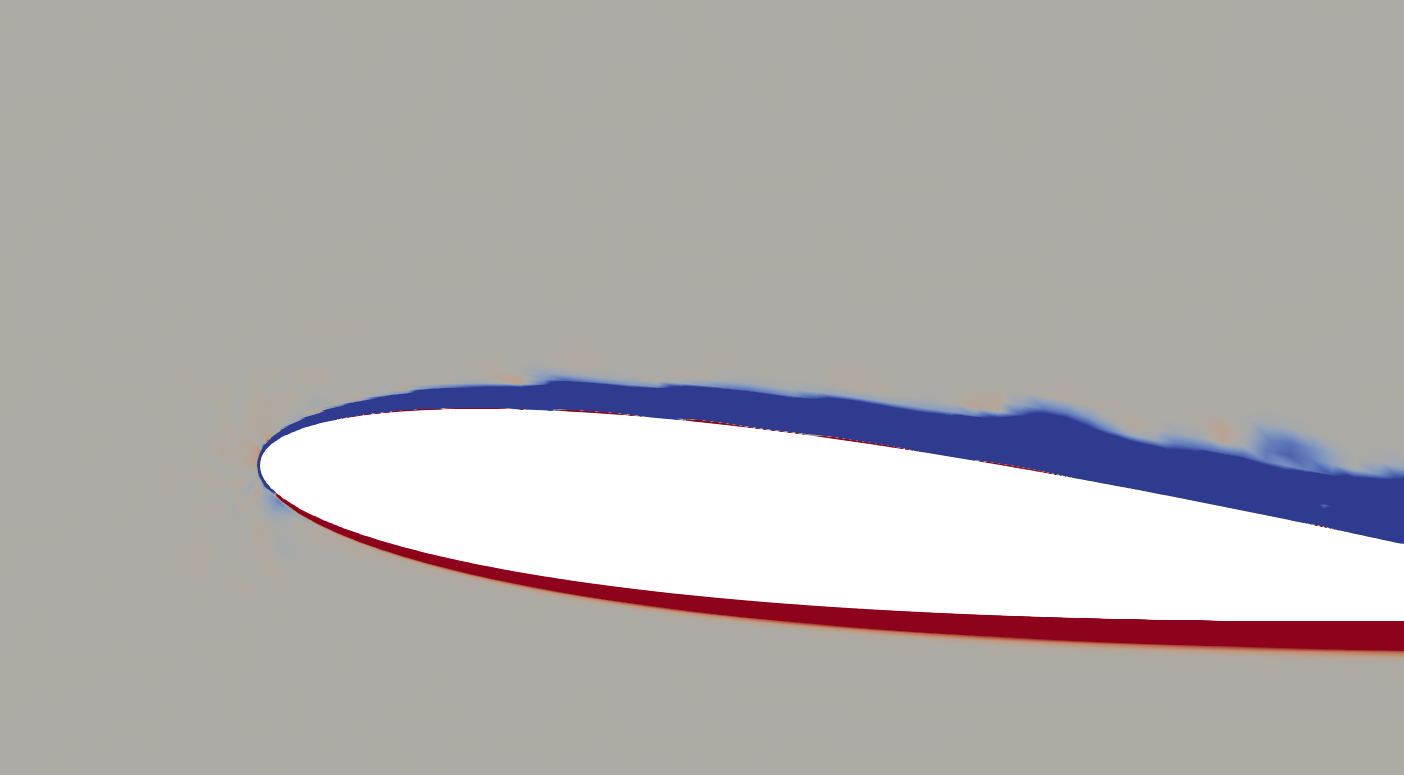
\includegraphics[width=1\textwidth]{figures/zonal_adapt_results/vorticity_plots/v2/M0/spavg/phase_180.png}
		\caption{M0 mesh, $\psi$ = $180^\circ$}
		\label{fig:M0_sp_psi180}
	\end{subfigure}
	\end{center}
	\begin{subfigure}[b]{0.475\textwidth}
	\centering
	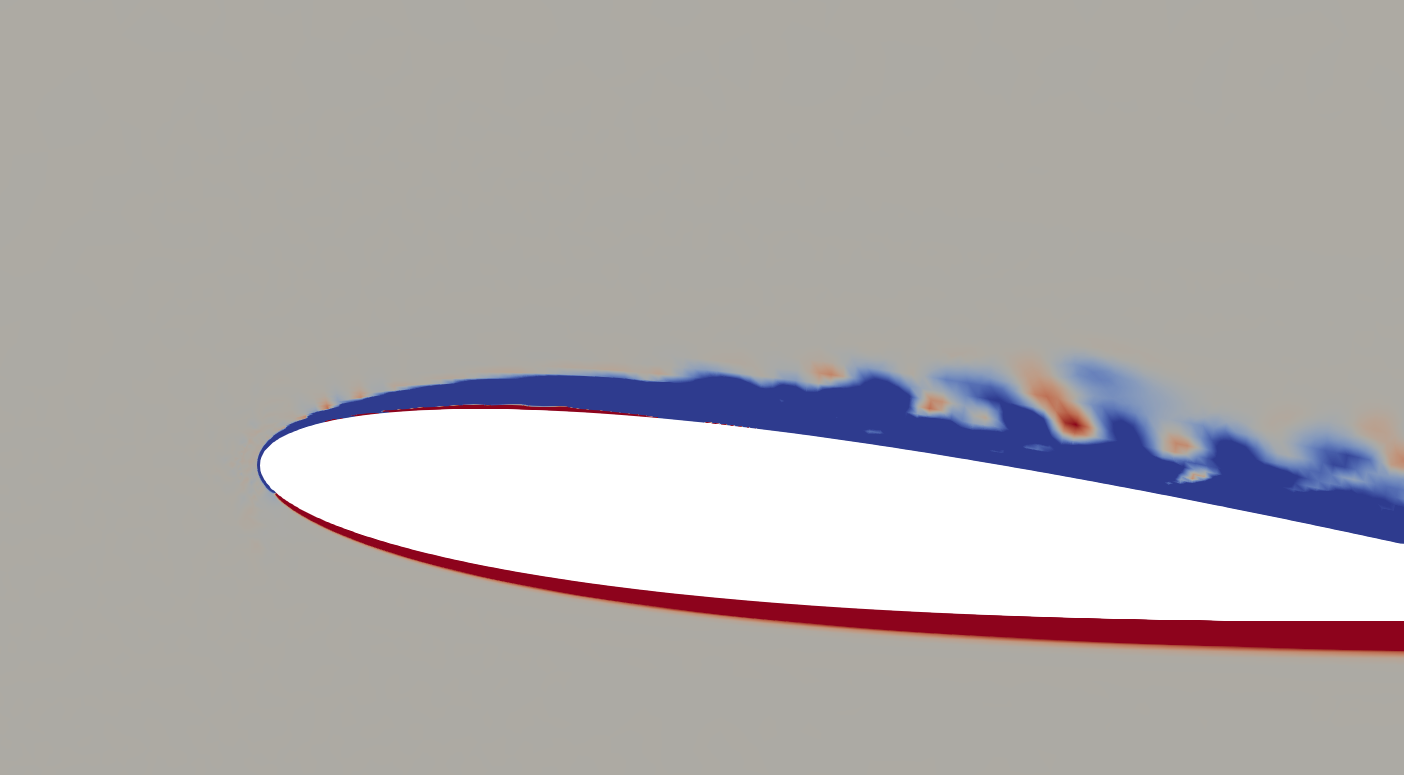
\includegraphics[width=1\textwidth]{figures/zonal_adapt_results/vorticity_plots/v2/Mza1_25/spavg/phase_180.png}
	\caption{Mza1\_25 mesh, $\psi$ = $180^\circ$}
	\label{fig:Mza1_25_sp_psi180}
\end{subfigure}
	\begin{subfigure}[b]{0.475\textwidth}
		\centering
		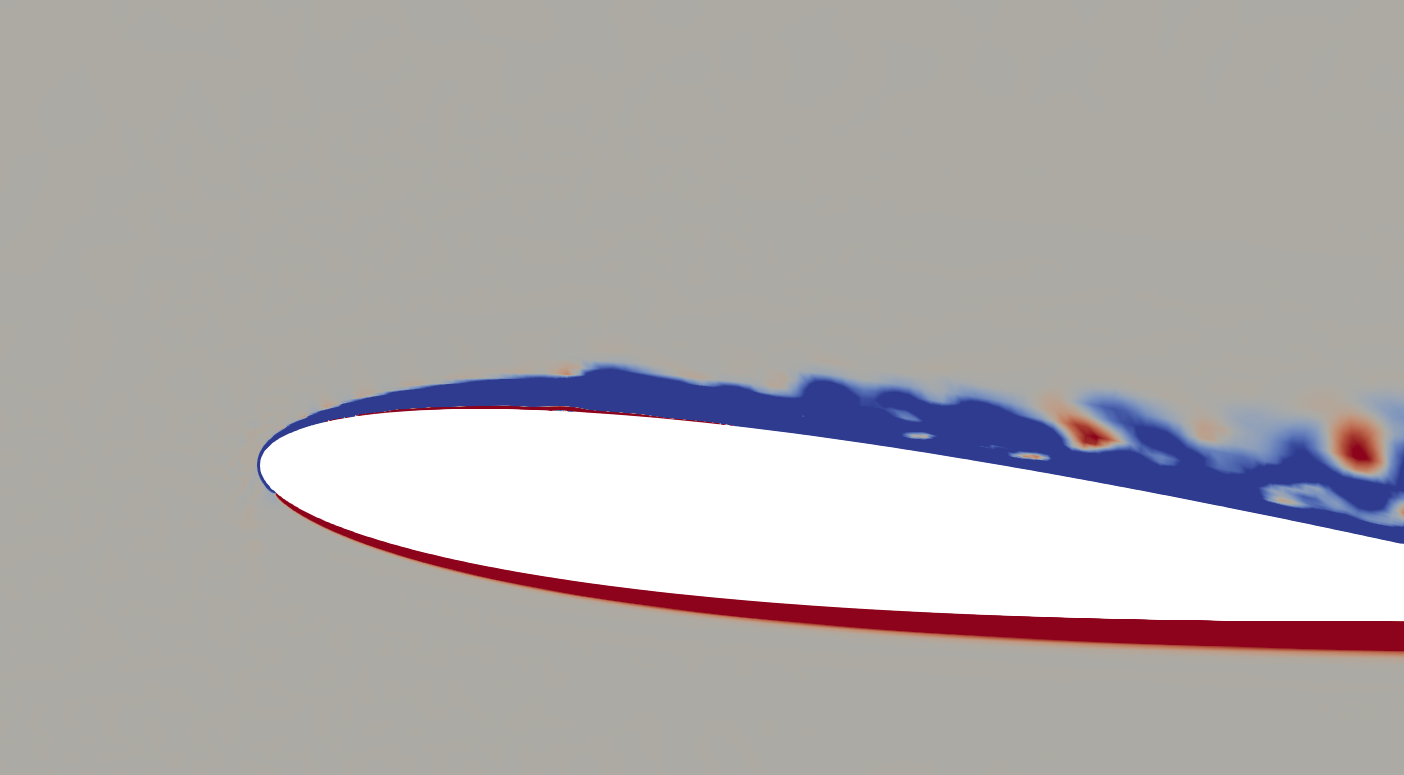
\includegraphics[width=1\textwidth]{figures/zonal_adapt_results/vorticity_plots/v2/Mza1_50/spavg/phase_180.png}
		\caption{Mza1\_50 mesh, $\psi$ = $180^\circ$}
		\label{fig:Mza1_50_sp_psi180}
	\end{subfigure}
%	\begin{subfigure}[b]{0.475\textwidth}
%		\centering
%		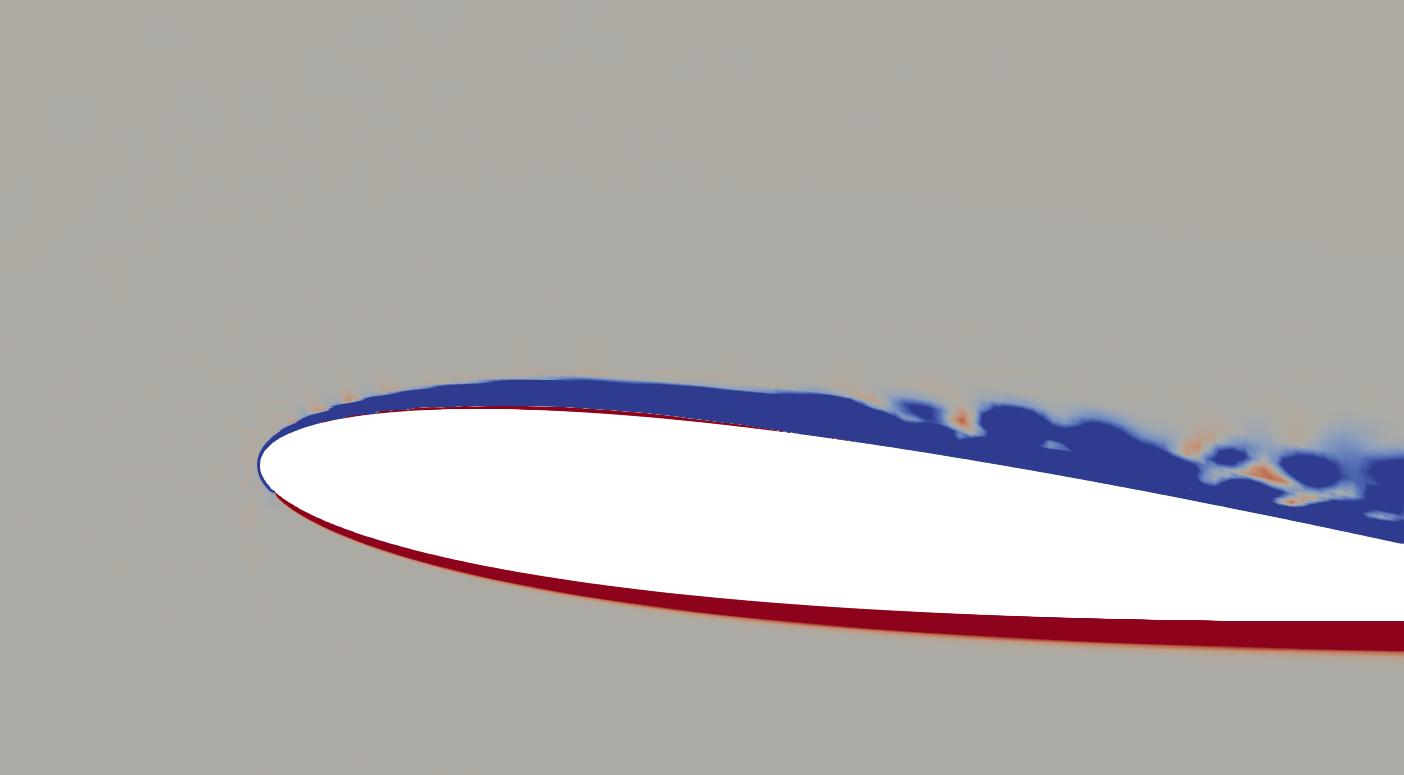
\includegraphics[width=1\textwidth]{figures/zonal_adapt_results/vorticity_plots/v2/Mza1_100/spavg/phase_180.png}
%		\caption{Mza1\_100 mesh, $\psi$ = $180^\circ$}
%		\label{fig:Mza1_100_sp_psi180}
%	\end{subfigure}
%	\begin{subfigure}[b]{0.475\textwidth}
%	\centering
%	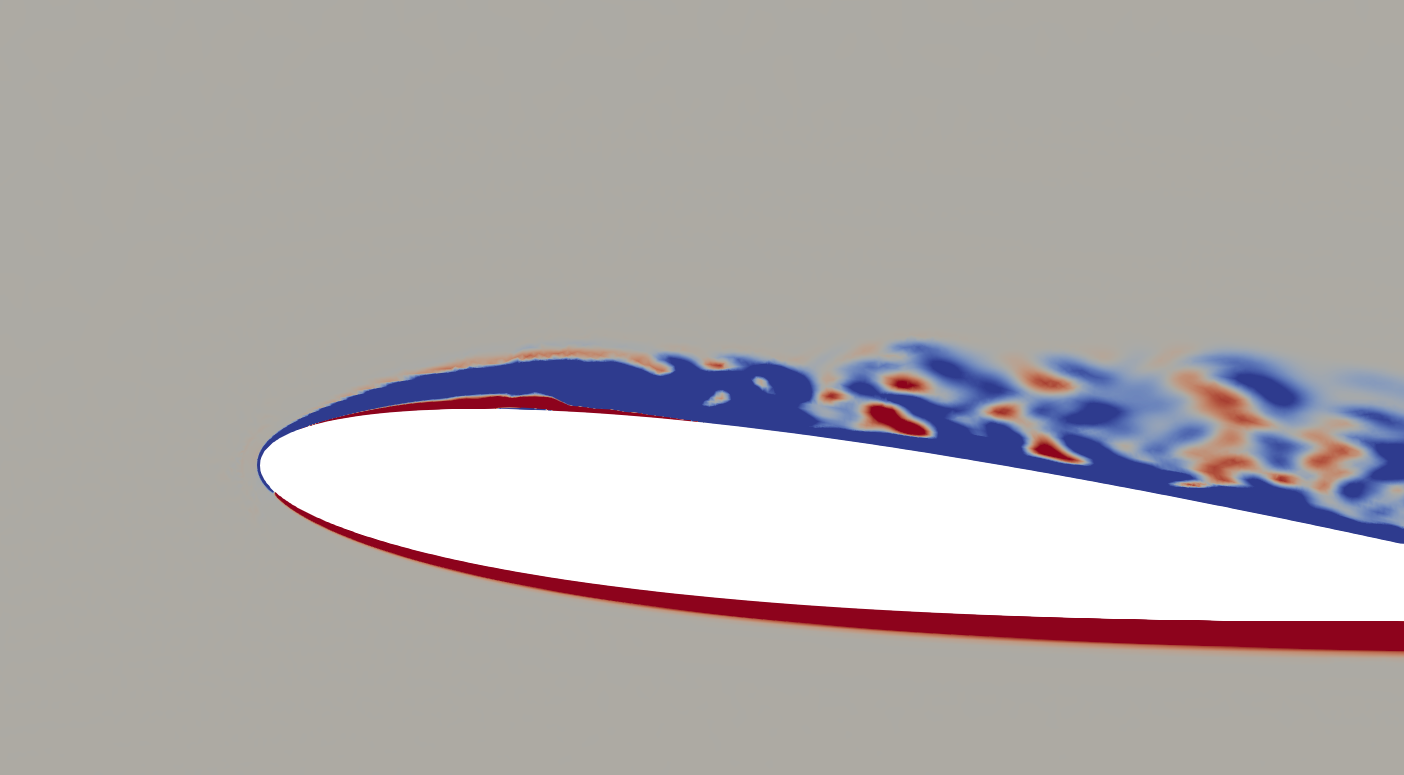
\includegraphics[width=1\textwidth]{figures/zonal_adapt_results/vorticity_plots/v2/Mza2_25/spavg/phase_180.png}
%	\caption{Mza2\_25 mesh, $\psi$ = $180^\circ$}
%	\label{fig:Mza2_25_sp_psi180}
%	\end{subfigure}
	\begin{subfigure}[b]{0.475\textwidth}
		\centering
		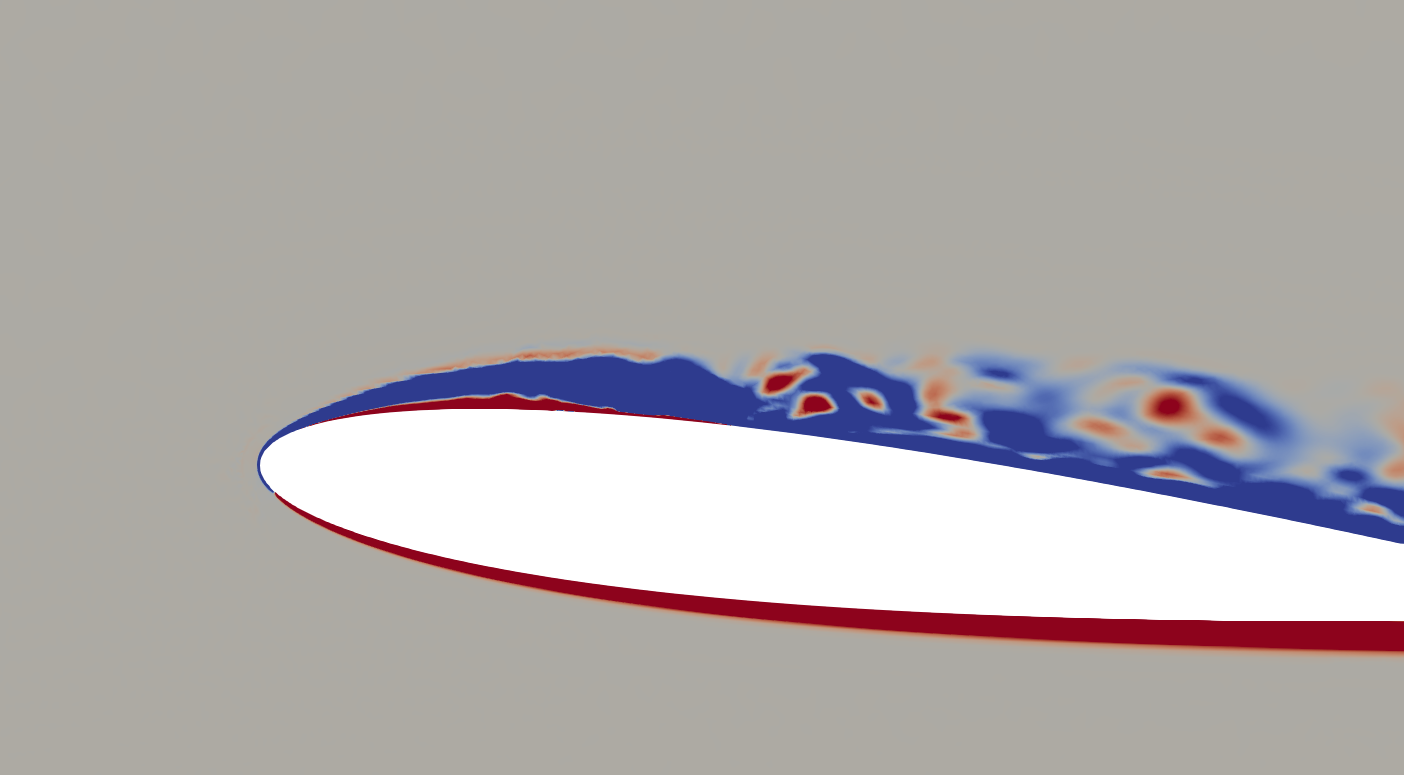
\includegraphics[width=1\textwidth]{figures/zonal_adapt_results/vorticity_plots/v2/Mza2_50/spavg/phase_180.png}
		\caption{Mza2\_50 mesh, $\psi$ = $180^\circ$}
		\label{fig:Mza2_50_sp_psi180}
	\end{subfigure}	
	\begin{subfigure}[b]{0.475\textwidth}
		\centering
		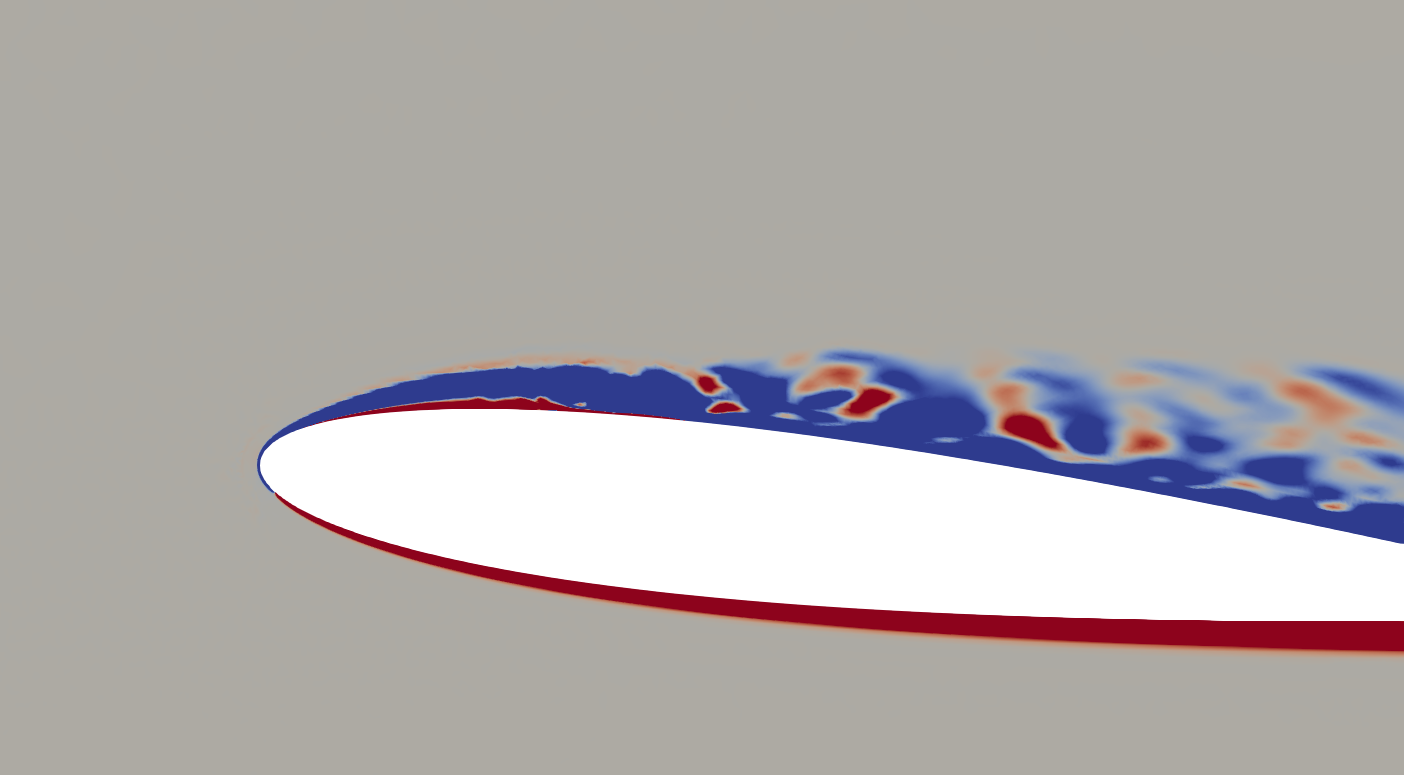
\includegraphics[width=1\textwidth]{figures/zonal_adapt_results/vorticity_plots/v2/Mza2_100/spavg/phase_180.png}
		\caption{Mza2\_100 mesh, $\psi$ = $180^\circ$}
		\label{fig:Mza2_100_sp_psi180}
	\end{subfigure}
	\begin{subfigure}[b]{0.475\textwidth}
	\centering
	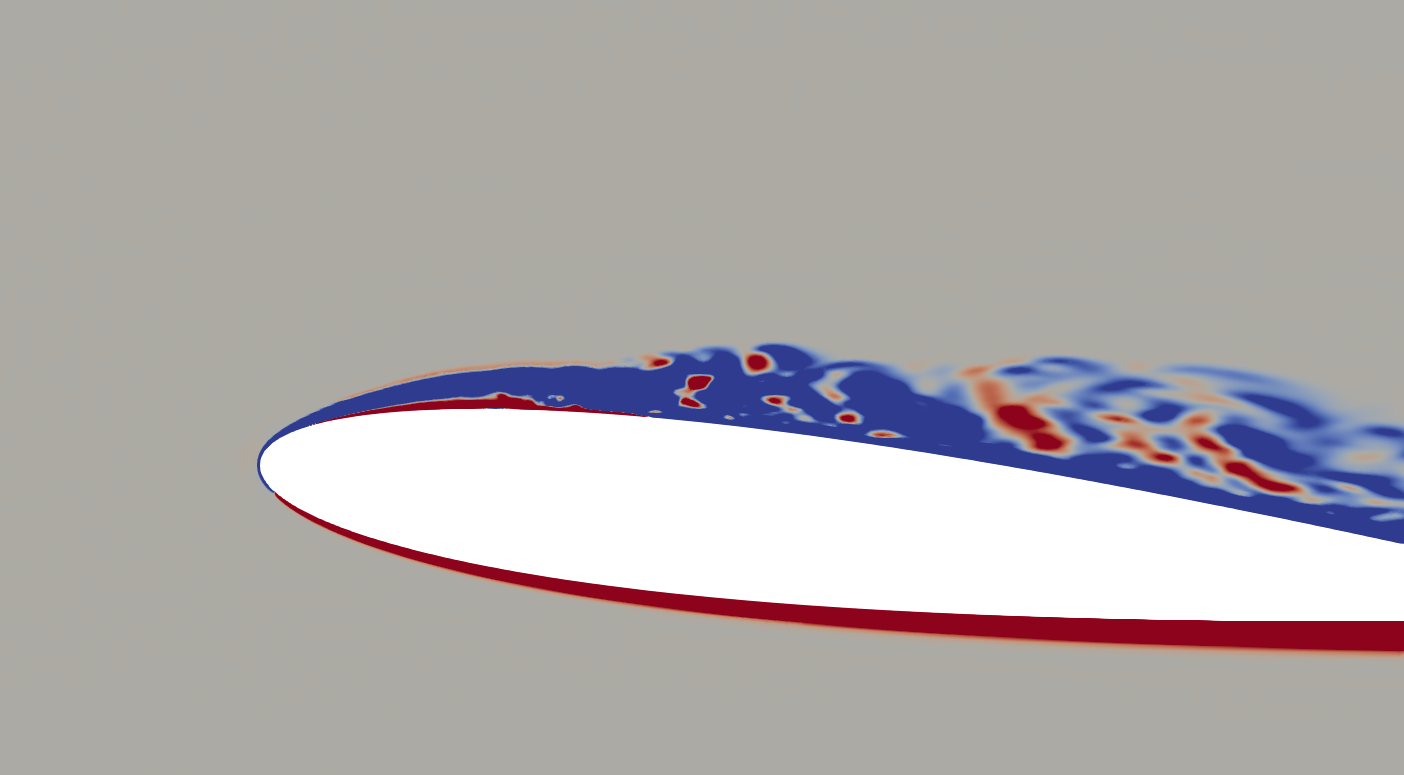
\includegraphics[width=1\textwidth]{figures/zonal_adapt_results/vorticity_plots/v2/Mza3_50/spavg/phase_180.png}
	\caption{Mza3\_50 mesh, $\psi$ = $180^\circ$}
	\label{fig:Mza3_100_sp_psi180}
	\end{subfigure}
	\begin{subfigure}[b]{0.475\textwidth}
		\centering
		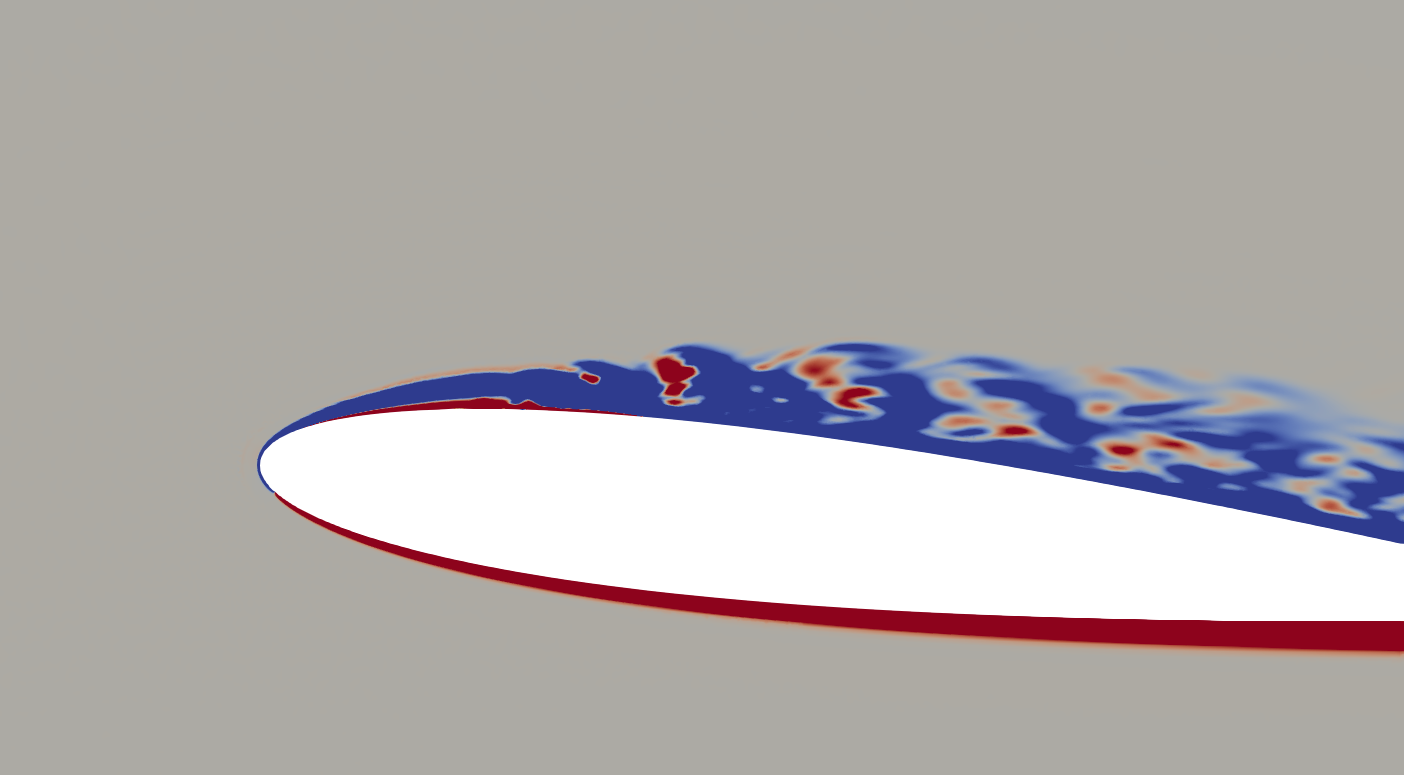
\includegraphics[width=1\textwidth]{figures/zonal_adapt_results/vorticity_plots/v2/Mza3_100/spavg/phase_180.png}
		\caption{Mza3\_100 mesh, $\psi$ = $180^\circ$}
		\label{fig:Mza3_100_sp_psi180}
	\end{subfigure}
	\caption{Spanwise vorticity comparison at $\psi$ = $180^\circ$ for different meshes}
	\label{fig:vorticity_sp_180}
\end{figure}

%%=====================================
%% Phase = 210
%%=====================================


\begin{figure}[H]
	\centering
	\begin{center}
		\begin{subfigure}[b]{0.475\textwidth}
		\centering
		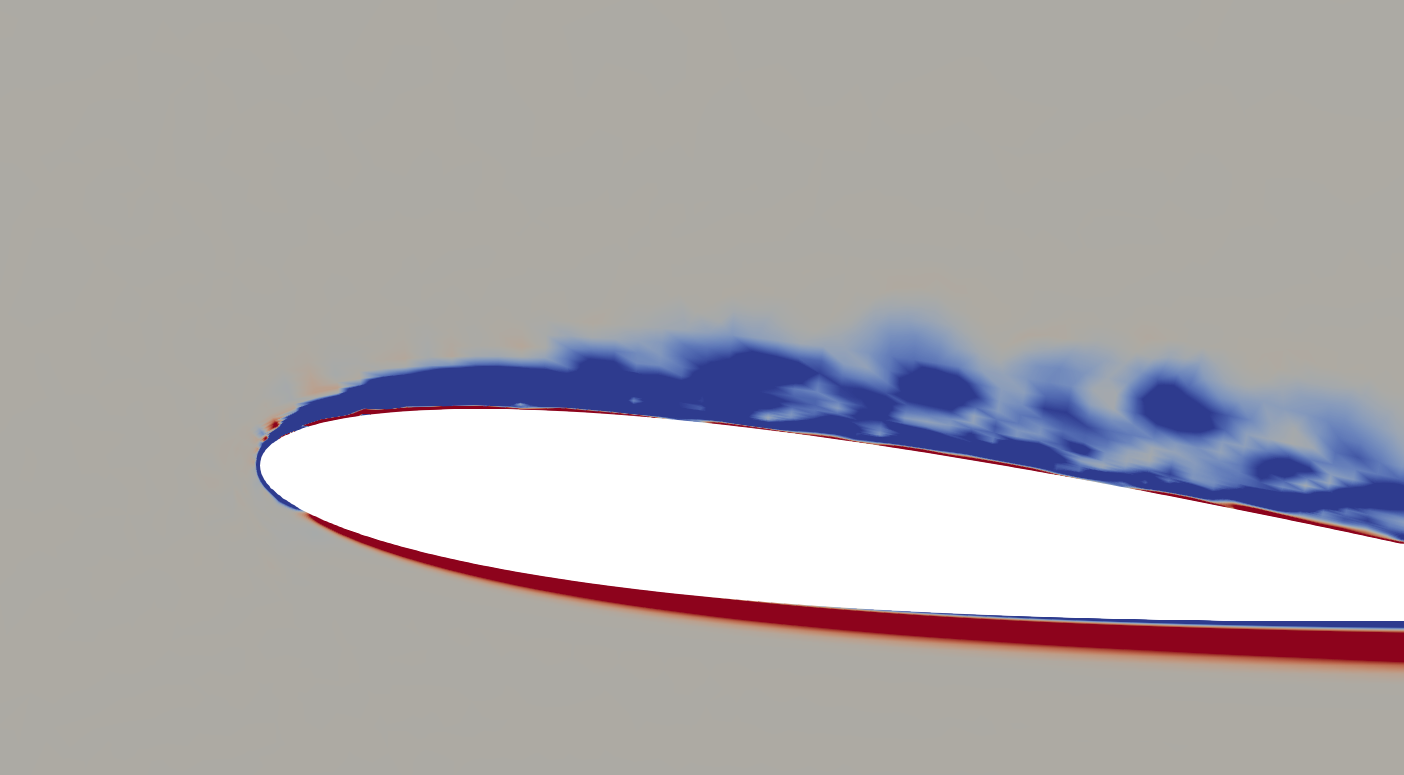
\includegraphics[width=1\textwidth]{figures/zonal_adapt_results/vorticity_plots/v2/M0/spavg/phase_210.png}
		\caption{M0 mesh, $\psi$ = $210^\circ$}
		\label{fig:M0_sp_psi210}
		\end{subfigure}
	\end{center}
	\begin{subfigure}[b]{0.475\textwidth}
	\centering
	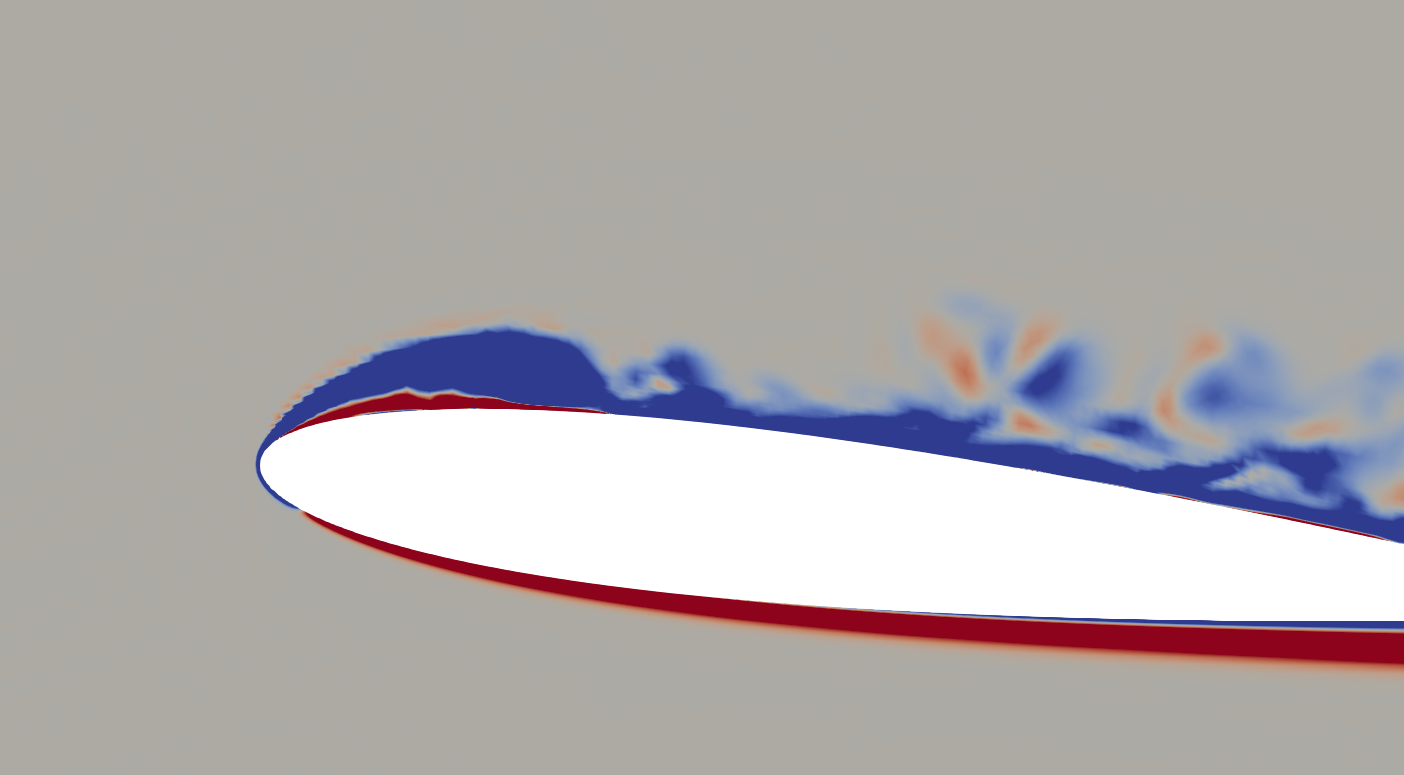
\includegraphics[width=1\textwidth]{figures/zonal_adapt_results/vorticity_plots/v2/Mza1_25/spavg/phase_210.png}
	\caption{Mza1\_25 mesh, $\psi$ = $210^\circ$}
	\label{fig:Mza1_25_sp_psi210}
	\end{subfigure}
	\begin{subfigure}[b]{0.475\textwidth}
		\centering
		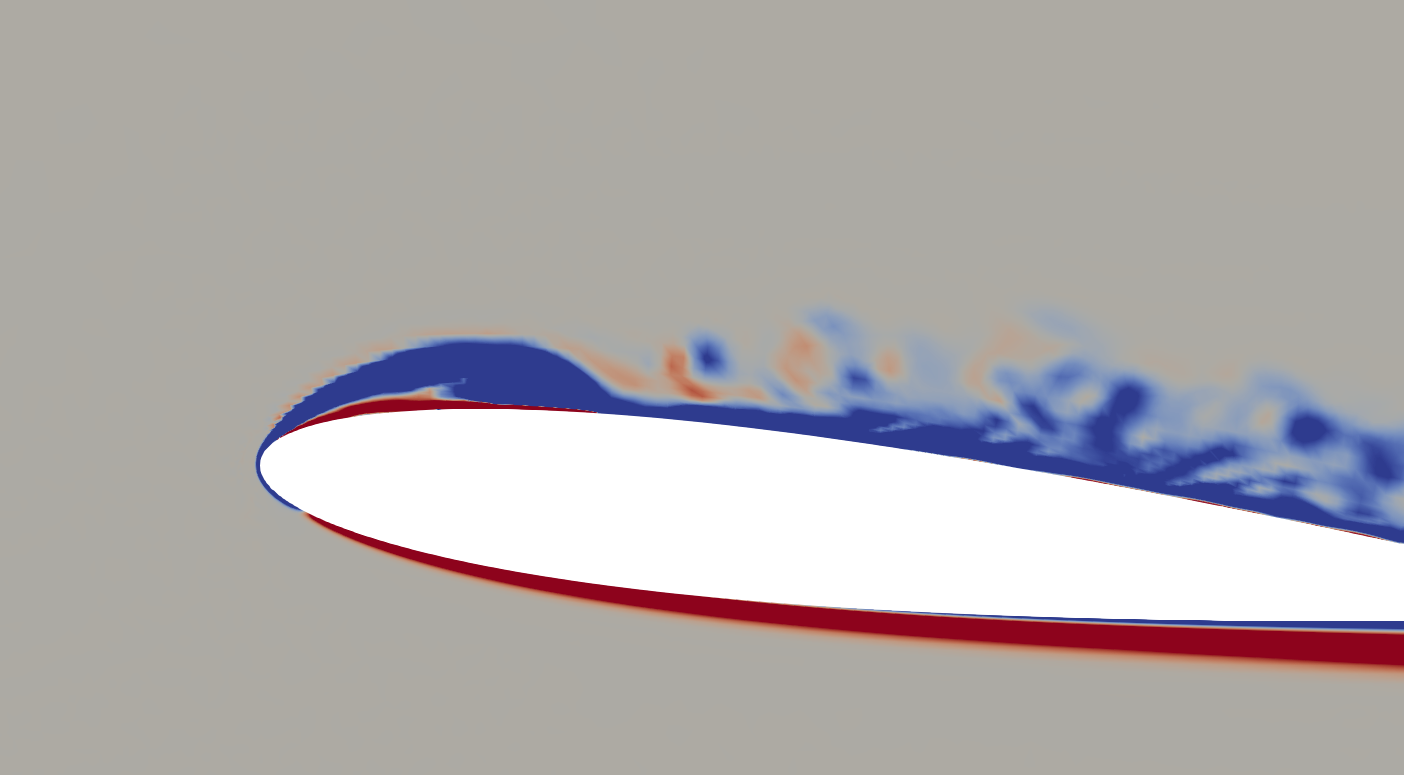
\includegraphics[width=1\textwidth]{figures/zonal_adapt_results/vorticity_plots/v2/Mza1_50/spavg/phase_210.png}
		\caption{Mza1\_50 mesh, $\psi$ = $210^\circ$}
		\label{fig:Mza1_50_sp_psi210}
	\end{subfigure}
%	\begin{subfigure}[b]{0.475\textwidth}
%		\centering
%		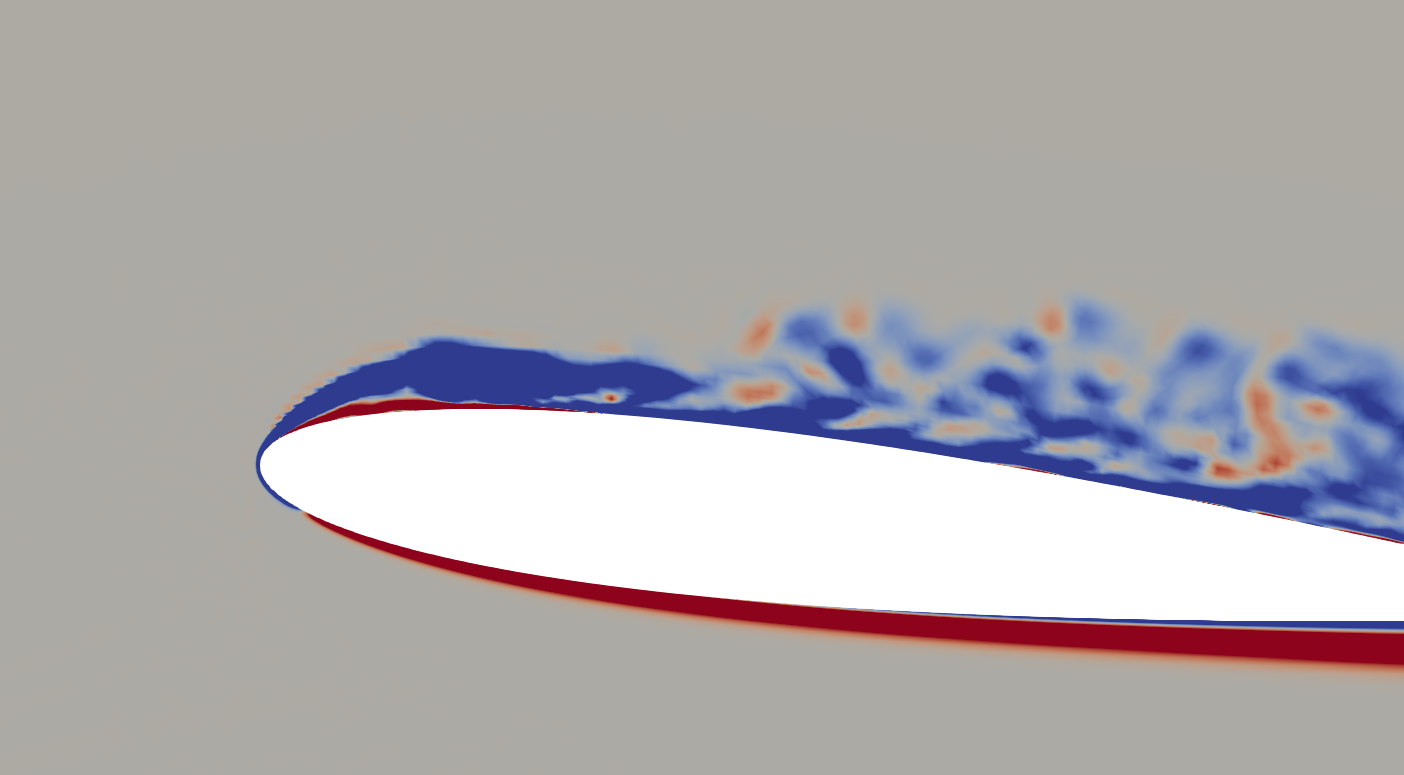
\includegraphics[width=1\textwidth]{figures/zonal_adapt_results/vorticity_plots/v2/Mza1_100/spavg/phase_210.png}
%		\caption{Mza1\_100 mesh, $\psi$ = $210^\circ$}
%		\label{fig:Mza1_100_sp_psi210}
%	\end{subfigure}
%	\begin{subfigure}[b]{0.475\textwidth}
%	\centering
%	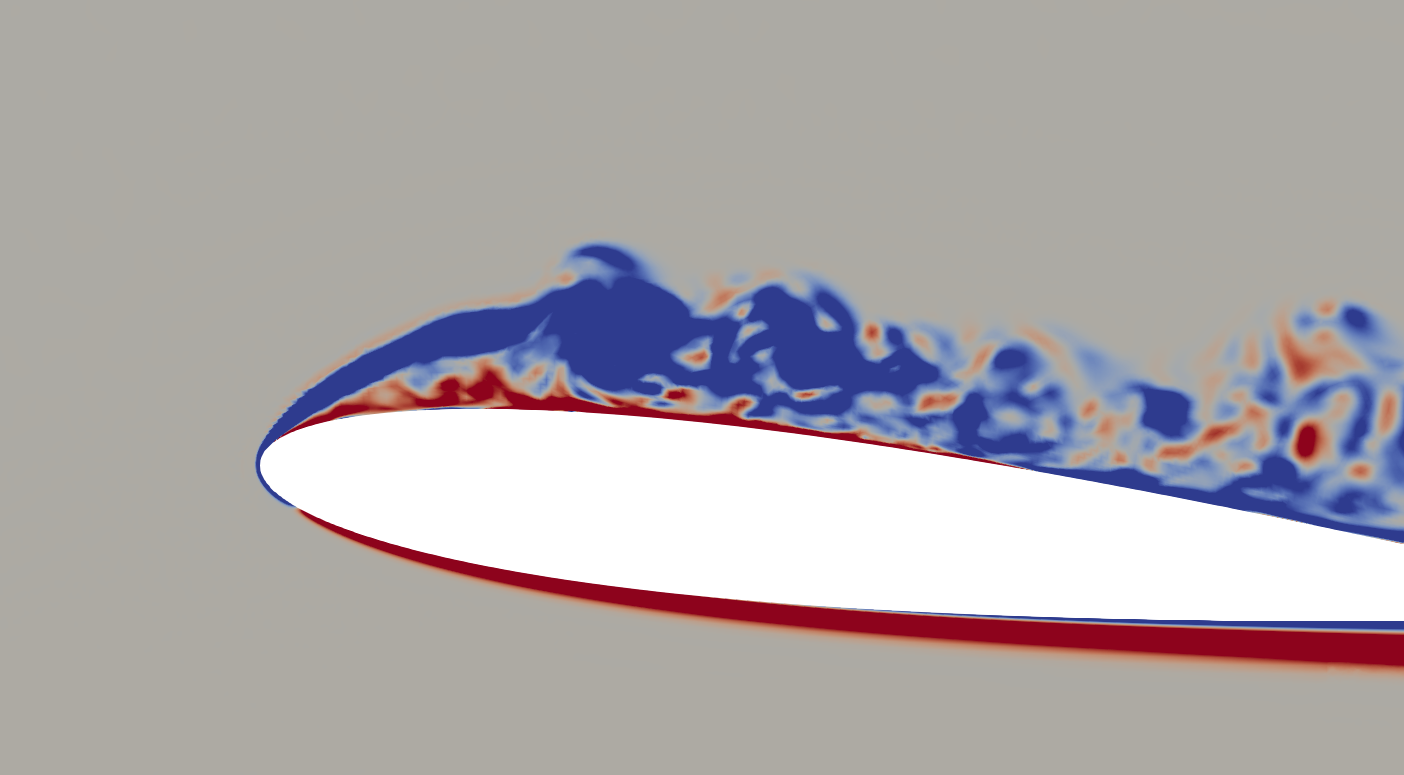
\includegraphics[width=1\textwidth]{figures/zonal_adapt_results/vorticity_plots/v2/Mza2_25/spavg/phase_210.png}
%	\caption{Mza2\_25 mesh, $\psi$ = $210^\circ$}
%	\label{fig:Mza2_25_sp_psi210}
%	\end{subfigure}	
	\begin{subfigure}[b]{0.475\textwidth}
		\centering
		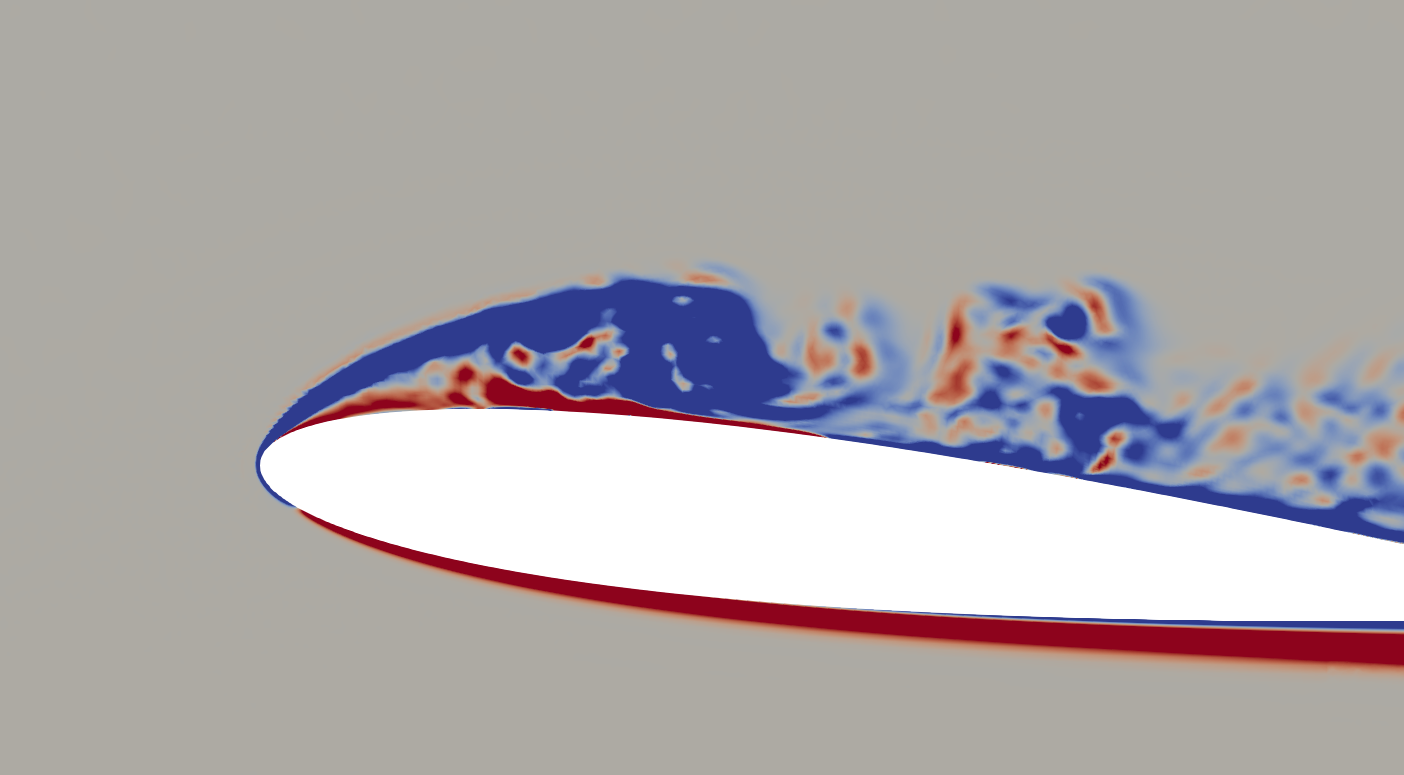
\includegraphics[width=1\textwidth]{figures/zonal_adapt_results/vorticity_plots/v2/Mza2_50/spavg/phase_210.png}
		\caption{Mza2\_50 mesh, $\psi$ = $210^\circ$}
		\label{fig:Mza2_50_sp_psi210}
	\end{subfigure}	
	\begin{subfigure}[b]{0.475\textwidth}
		\centering
		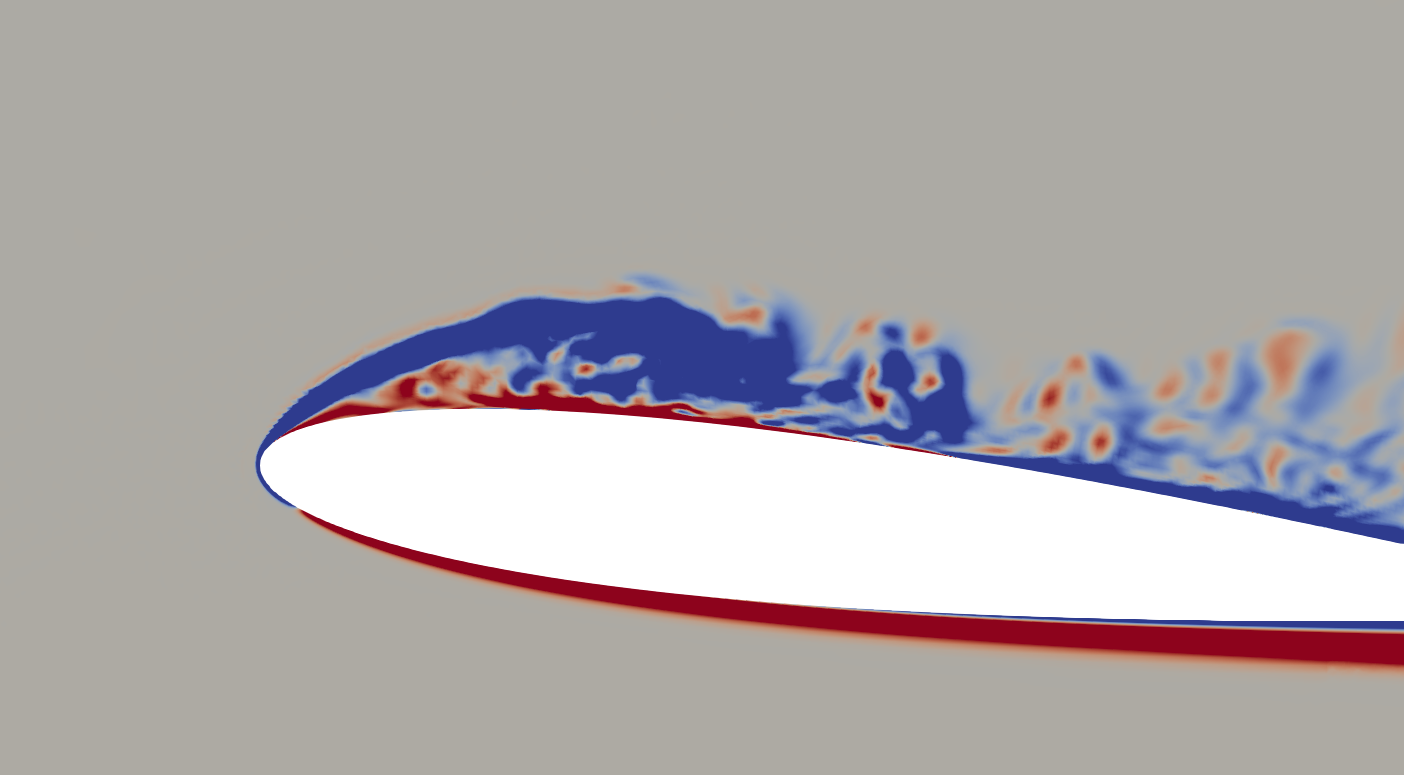
\includegraphics[width=1\textwidth]{figures/zonal_adapt_results/vorticity_plots/v2/Mza2_100/spavg/phase_210.png}
		\caption{Mza2\_100 mesh, $\psi$ = $210^\circ$}
		\label{fig:Mza2_100_sp_psi210}
	\end{subfigure}
	\begin{subfigure}[b]{0.475\textwidth}
	\centering
	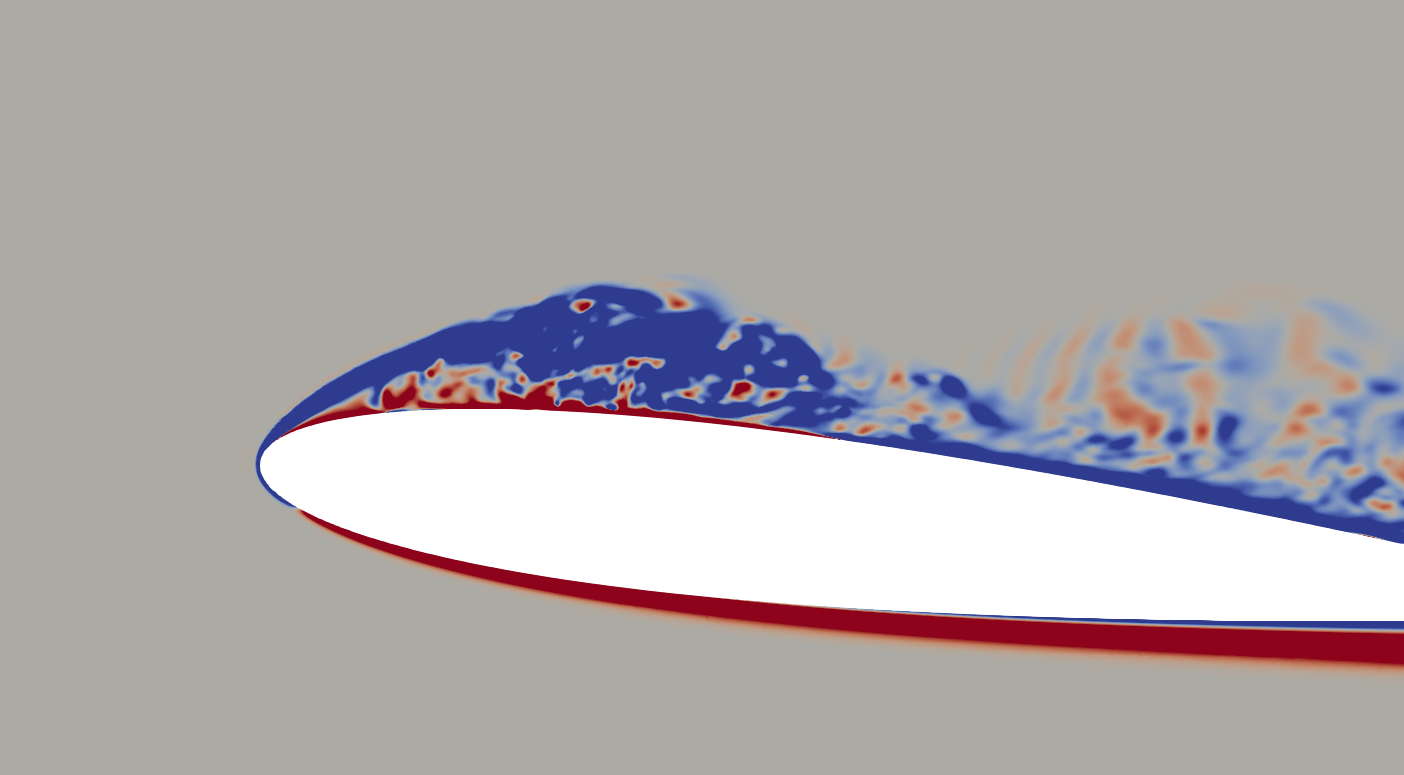
\includegraphics[width=1\textwidth]{figures/zonal_adapt_results/vorticity_plots/v2/Mza3_50/spavg/phase_210.png}
	\caption{Mza3\_50 mesh, $\psi$ = $210^\circ$}
	\label{fig:Mza3_50_sp_psi210}
\end{subfigure}
	\begin{subfigure}[b]{0.475\textwidth}
		\centering
		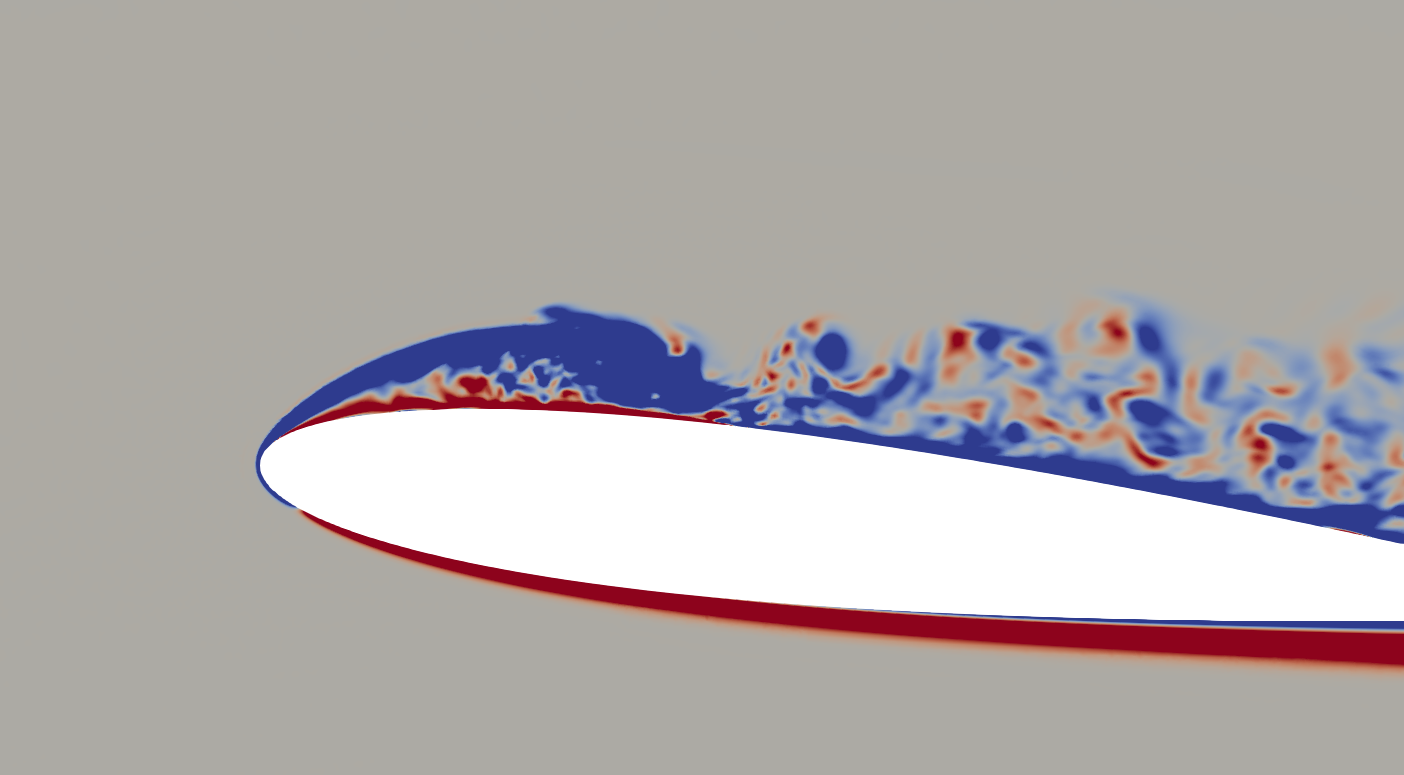
\includegraphics[width=1\textwidth]{figures/zonal_adapt_results/vorticity_plots/v2/Mza3_100/spavg/phase_210.png}
		\caption{Mza3\_100 mesh, $\psi$ = $210^\circ$}
		\label{fig:Mza3_100_sp_psi210}
	\end{subfigure}
	\caption{Spanwise vorticity comparison at $\psi$ = $210^\circ$ for different meshes}
	\label{fig:vorticity_sp_210}
\end{figure}

%%=====================================
%% Phase = 240
%%=====================================


\begin{figure}[H]
	\centering
	\begin{center}
		\begin{subfigure}[b]{0.475\textwidth}
		\centering
		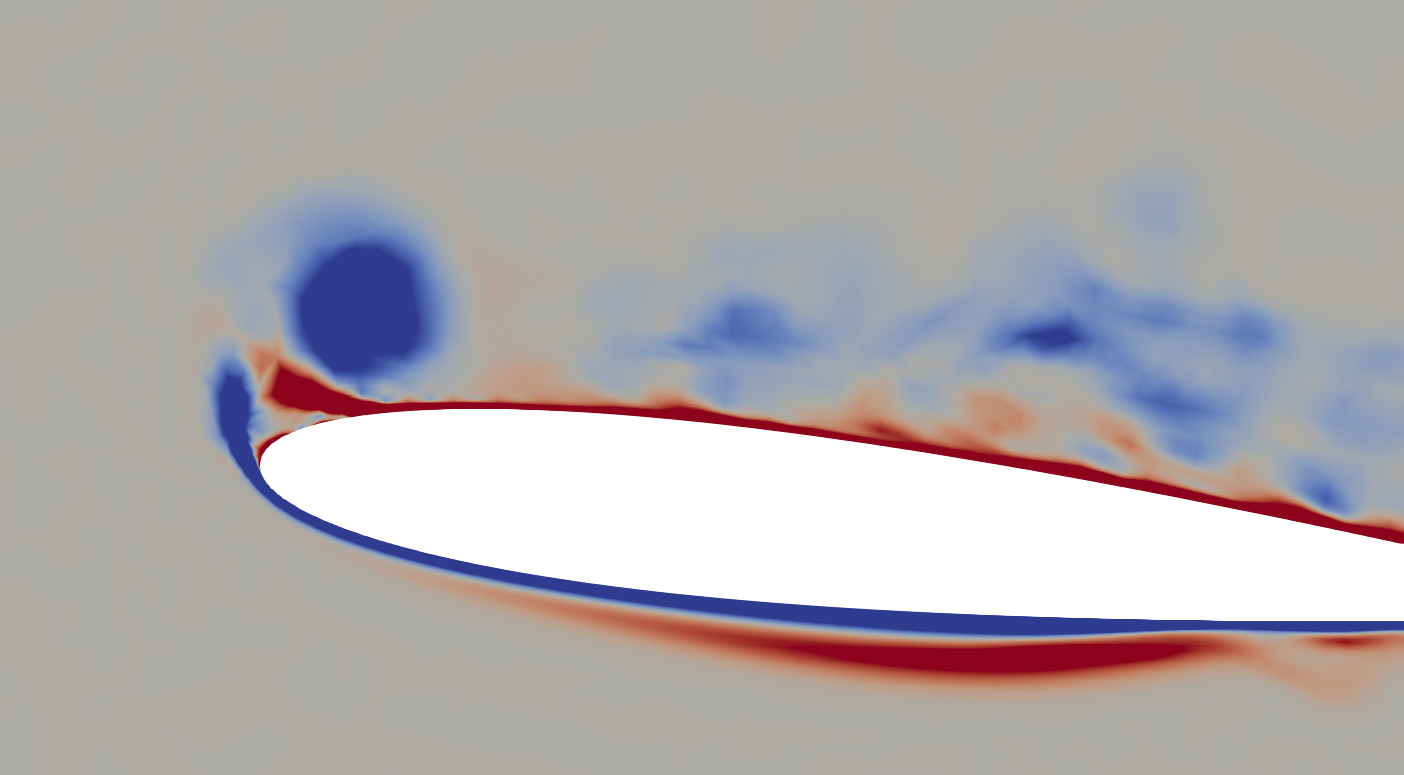
\includegraphics[width=1\textwidth]{figures/zonal_adapt_results/vorticity_plots/v2/M0/spavg/phase_240.png}
		\caption{M0 mesh, $\psi$ = $240^\circ$}
		\label{fig:M0_sp_psi240}
		\end{subfigure}
	\end{center}
	\begin{subfigure}[b]{0.475\textwidth}
		\centering
		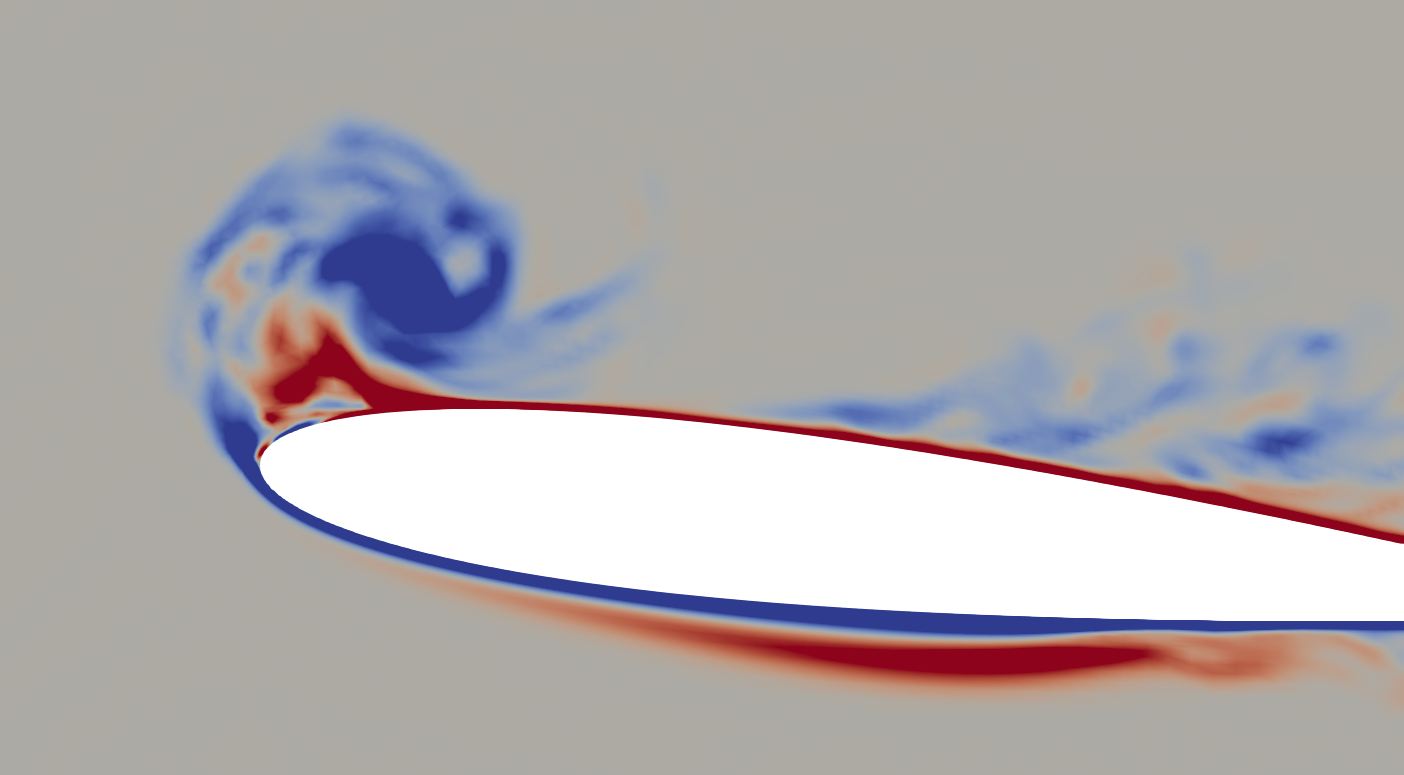
\includegraphics[width=1\textwidth]{figures/zonal_adapt_results/vorticity_plots/v2/Mza1_25/spavg/phase_240.png}
		\caption{Mza1\_25 mesh, $\psi$ = $240^\circ$}
		\label{fig:Mza1_25_sp_psi240}
	\end{subfigure}
	\begin{subfigure}[b]{0.475\textwidth}
	\centering
	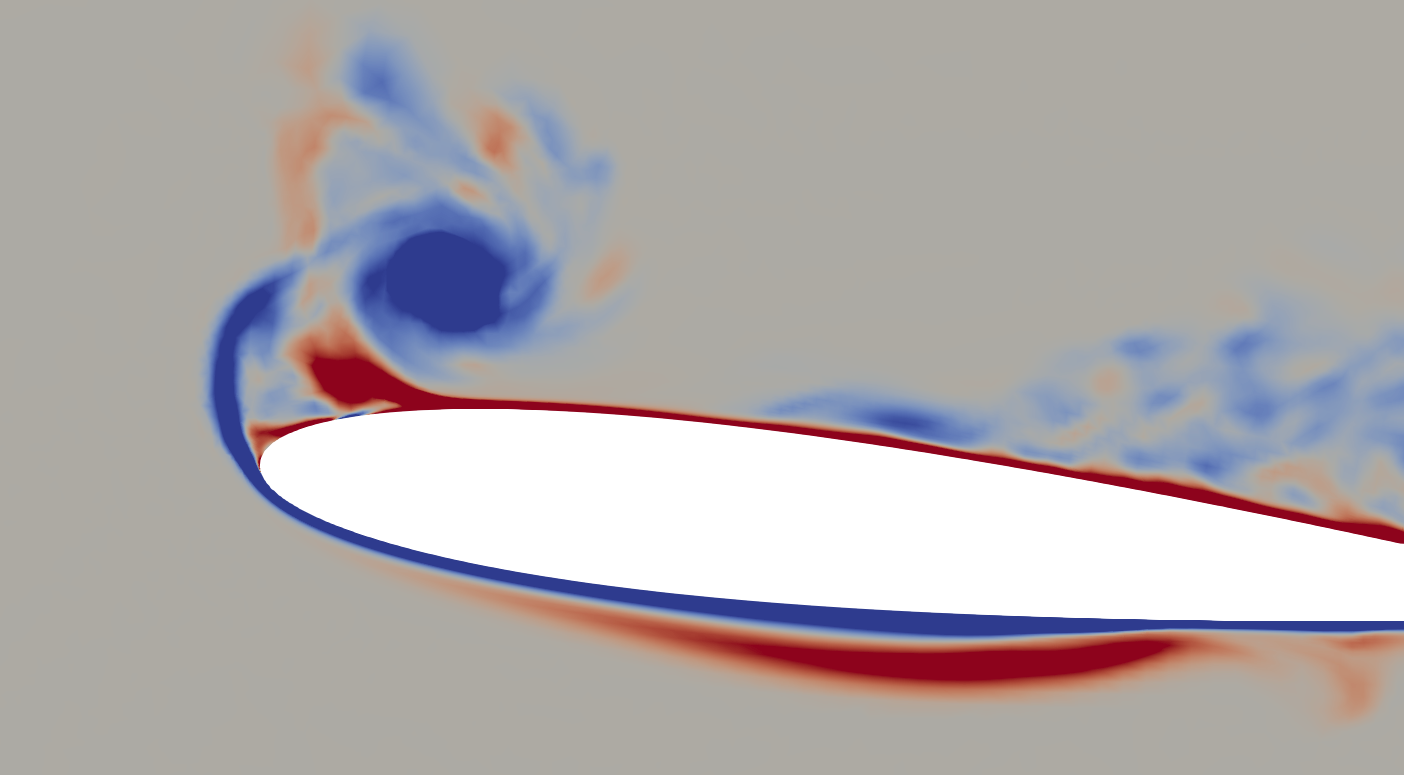
\includegraphics[width=1\textwidth]{figures/zonal_adapt_results/vorticity_plots/v2/Mza1_50/spavg/phase_240.png}
	\caption{Mza1\_50 mesh, $\psi$ = $240^\circ$}
	\label{fig:Mza1_50_sp_psi240}
	\end{subfigure}
	\begin{subfigure}[b]{0.475\textwidth}
		\centering
		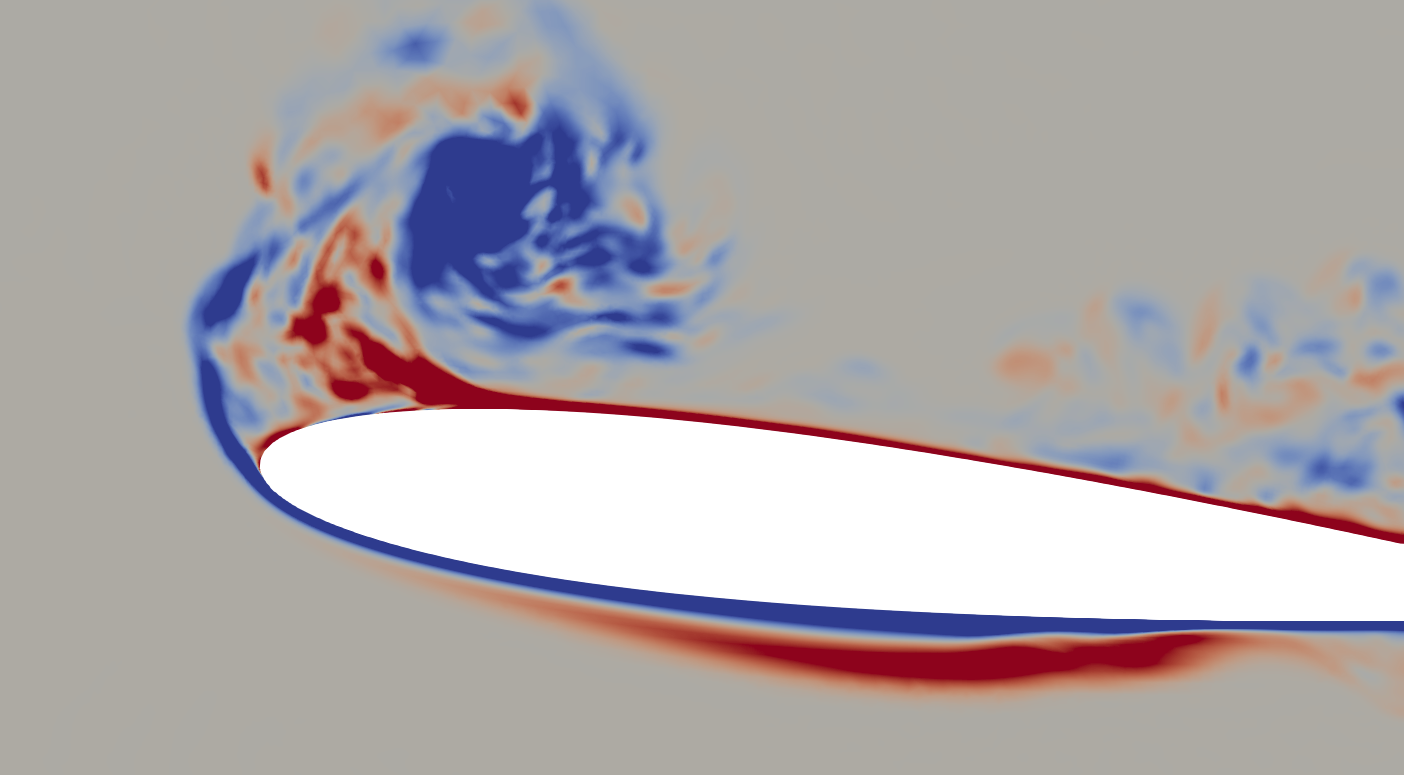
\includegraphics[width=1\textwidth]{figures/zonal_adapt_results/vorticity_plots/v2/Mza2_50/spavg/phase_240.png}
		\caption{Mza2\_50 mesh, $\psi$ = $240^\circ$}
		\label{fig:Mza2_50_sp_psi240}
	\end{subfigure}
%	\begin{subfigure}[b]{0.475\textwidth}
%		\centering
%		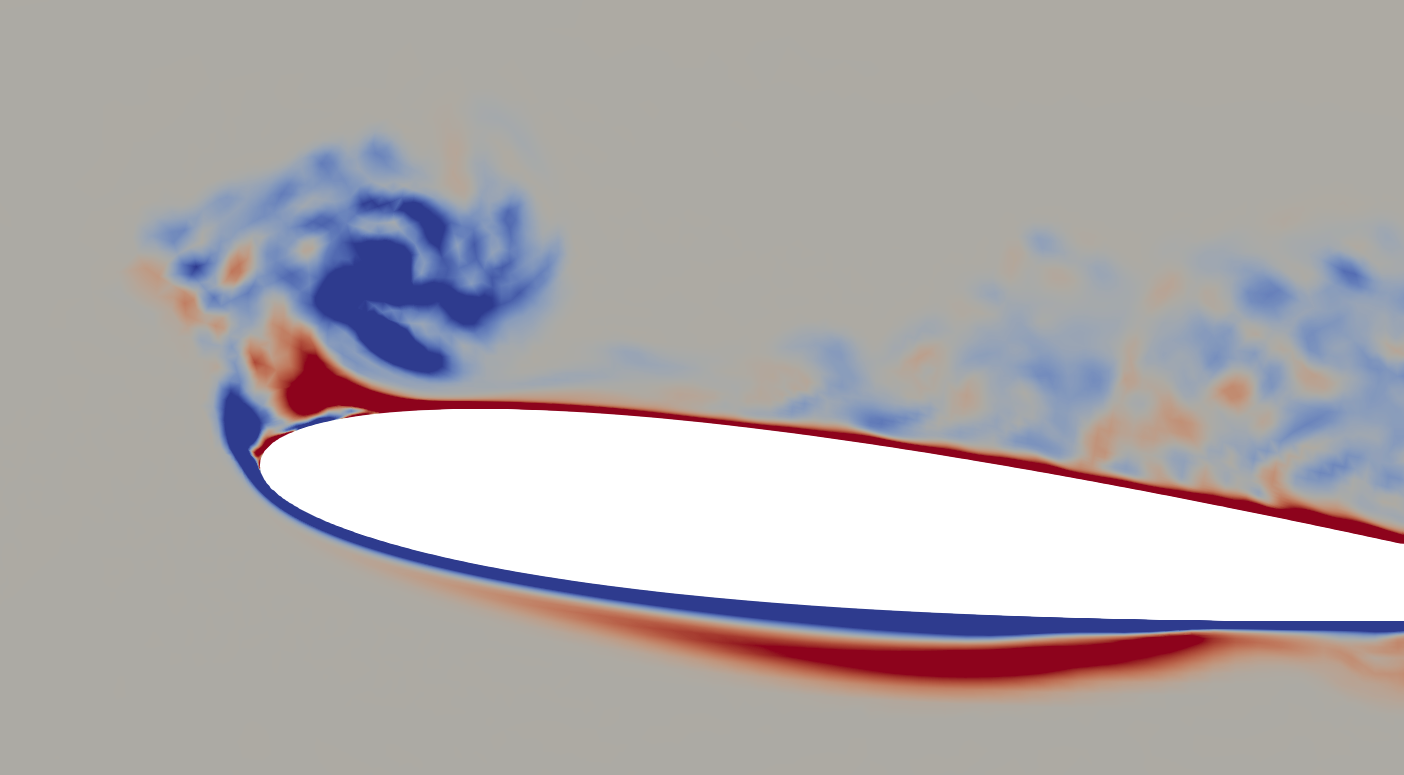
\includegraphics[width=1\textwidth]{figures/zonal_adapt_results/vorticity_plots/v2/Mza1_100/spavg/phase_240.png}
%		\caption{Mza1\_100 mesh, $\psi$ = $240^\circ$}
%		\label{fig:Mza1_100_sp_psi240}
%	\end{subfigure}
%	\begin{subfigure}[b]{0.475\textwidth}
%	\centering
%	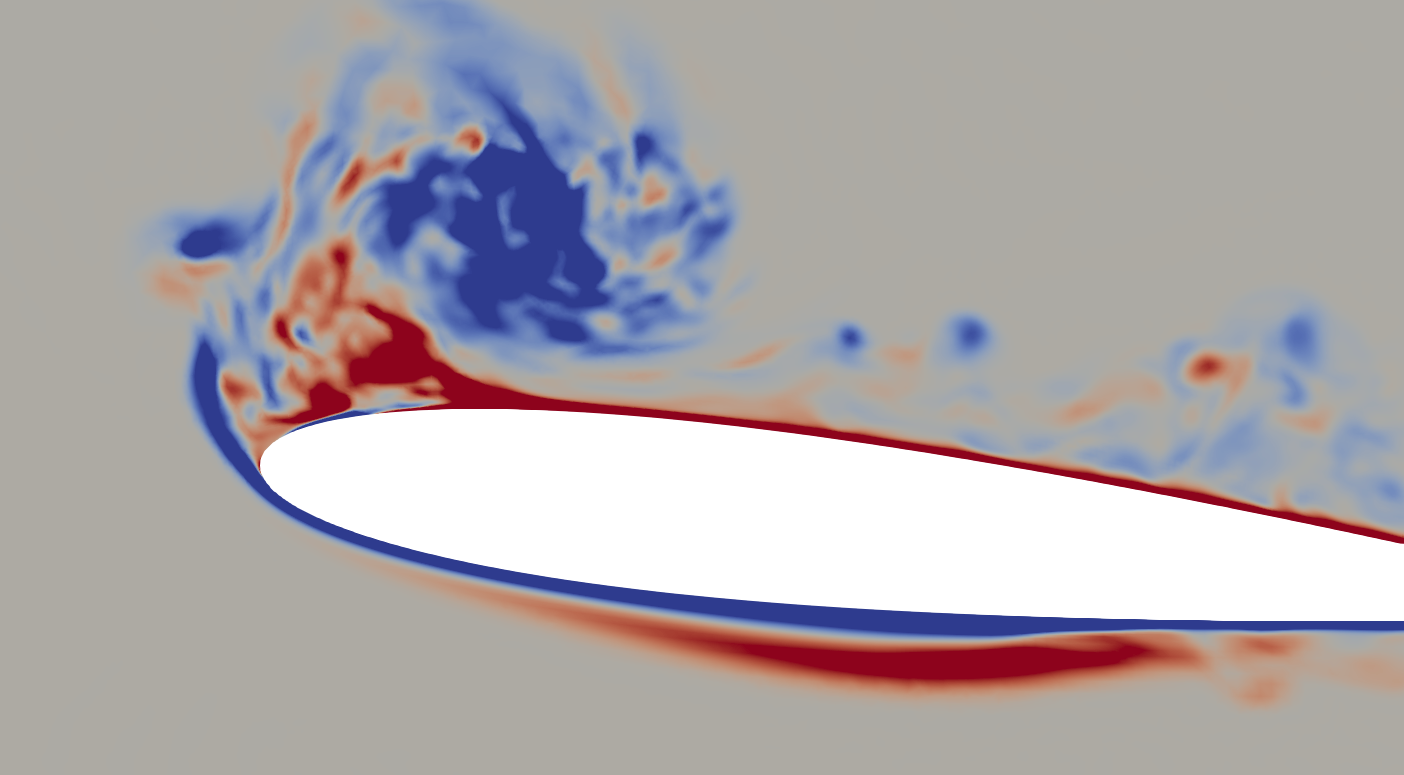
\includegraphics[width=1\textwidth]{figures/zonal_adapt_results/vorticity_plots/v2/Mza2_25/spavg/phase_240.png}
%	\caption{Mza2\_25 mesh, $\psi$ = $240^\circ$}
%	\label{fig:Mza2_25_sp_psi240}
%	\end{subfigure}	
%	\begin{subfigure}[b]{0.475\textwidth}
%		\centering
%		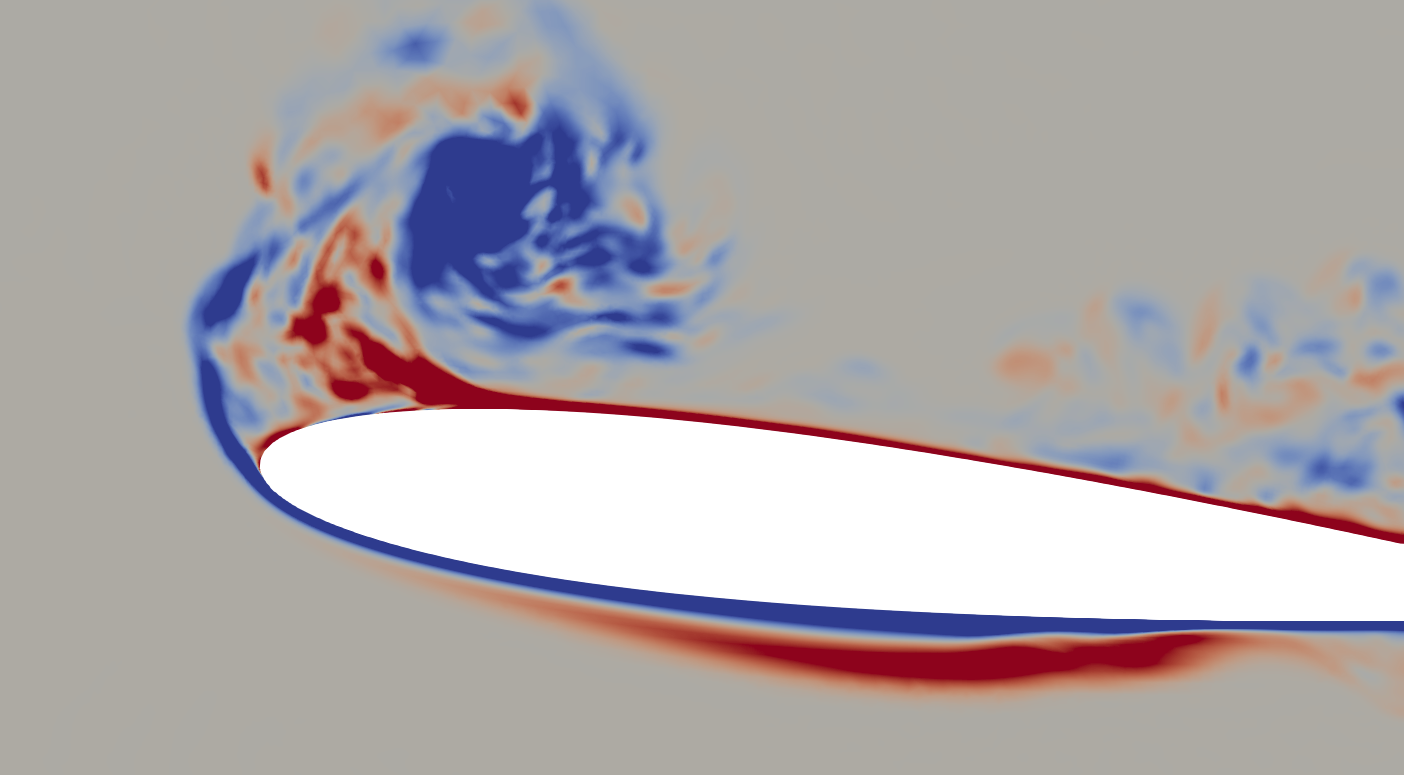
\includegraphics[width=1\textwidth]{figures/zonal_adapt_results/vorticity_plots/v2/Mza2_50/spavg/phase_240.png}
%		\caption{Mza2\_50 mesh, $\psi$ = $240^\circ$}
%		\label{fig:Mza2_50_sp_psi240}
%	\end{subfigure}	
	\begin{subfigure}[b]{0.475\textwidth}
		\centering
		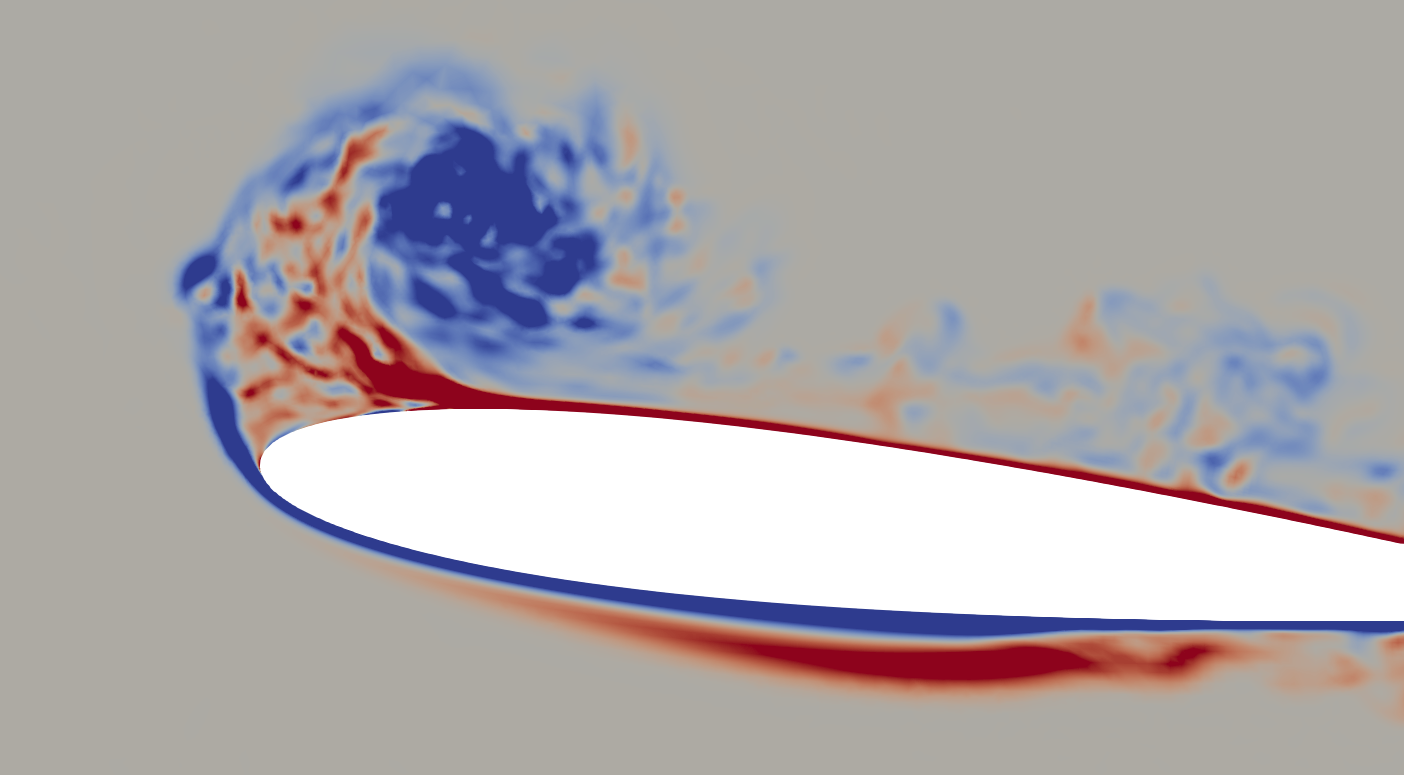
\includegraphics[width=1\textwidth]{figures/zonal_adapt_results/vorticity_plots/v2/Mza2_100/spavg/phase_240.png}
		\caption{Mza2\_100 mesh, $\psi$ = $240^\circ$}
		\label{fig:Mza2_100_sp_psi240}
	\end{subfigure}
	\begin{subfigure}[b]{0.475\textwidth}
	\centering
	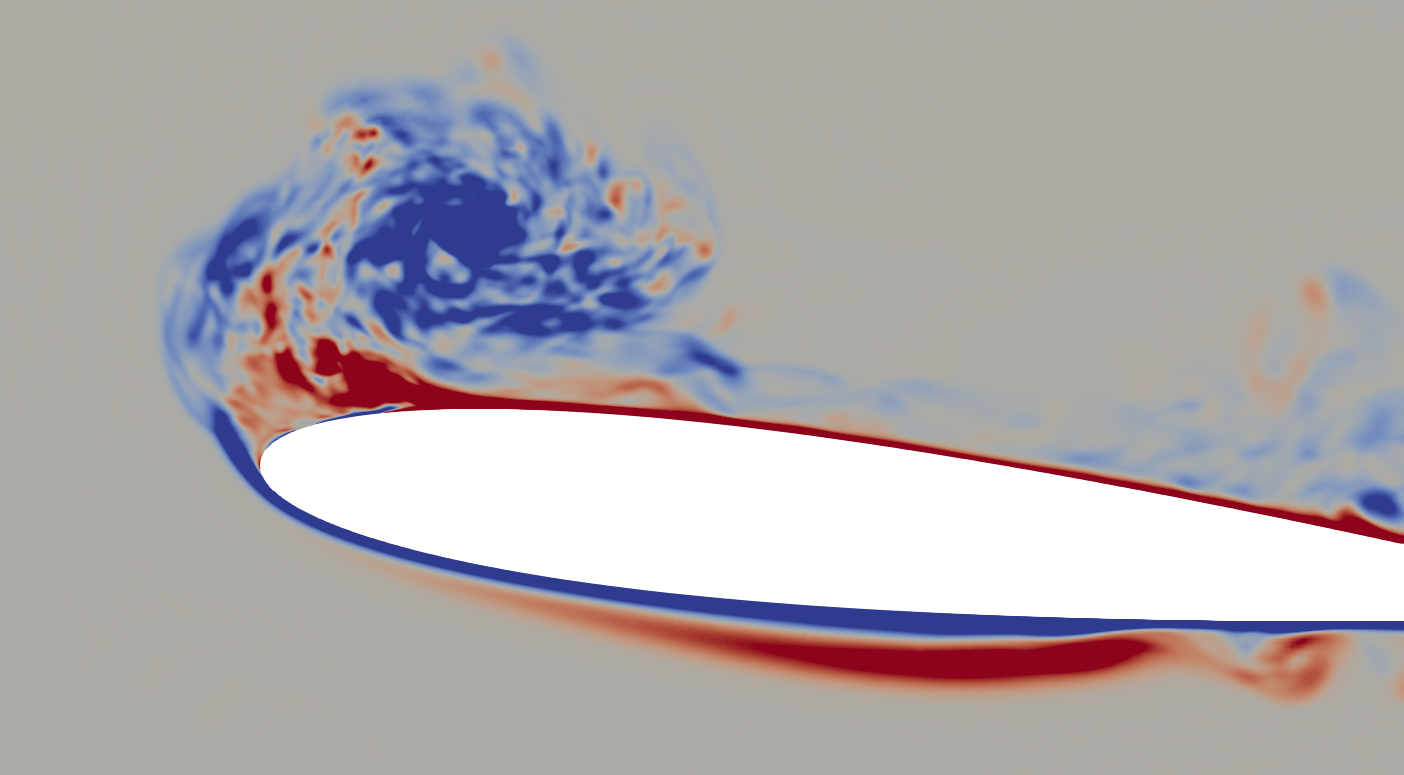
\includegraphics[width=1\textwidth]{figures/zonal_adapt_results/vorticity_plots/v2/Mza3_50/spavg/phase_240.png}
	\caption{Mza3\_50 mesh, $\psi$ = $240^\circ$}
	\label{fig:Mza3_100_sp_psi240}
\end{subfigure}
	\begin{subfigure}[b]{0.475\textwidth}
		\centering
		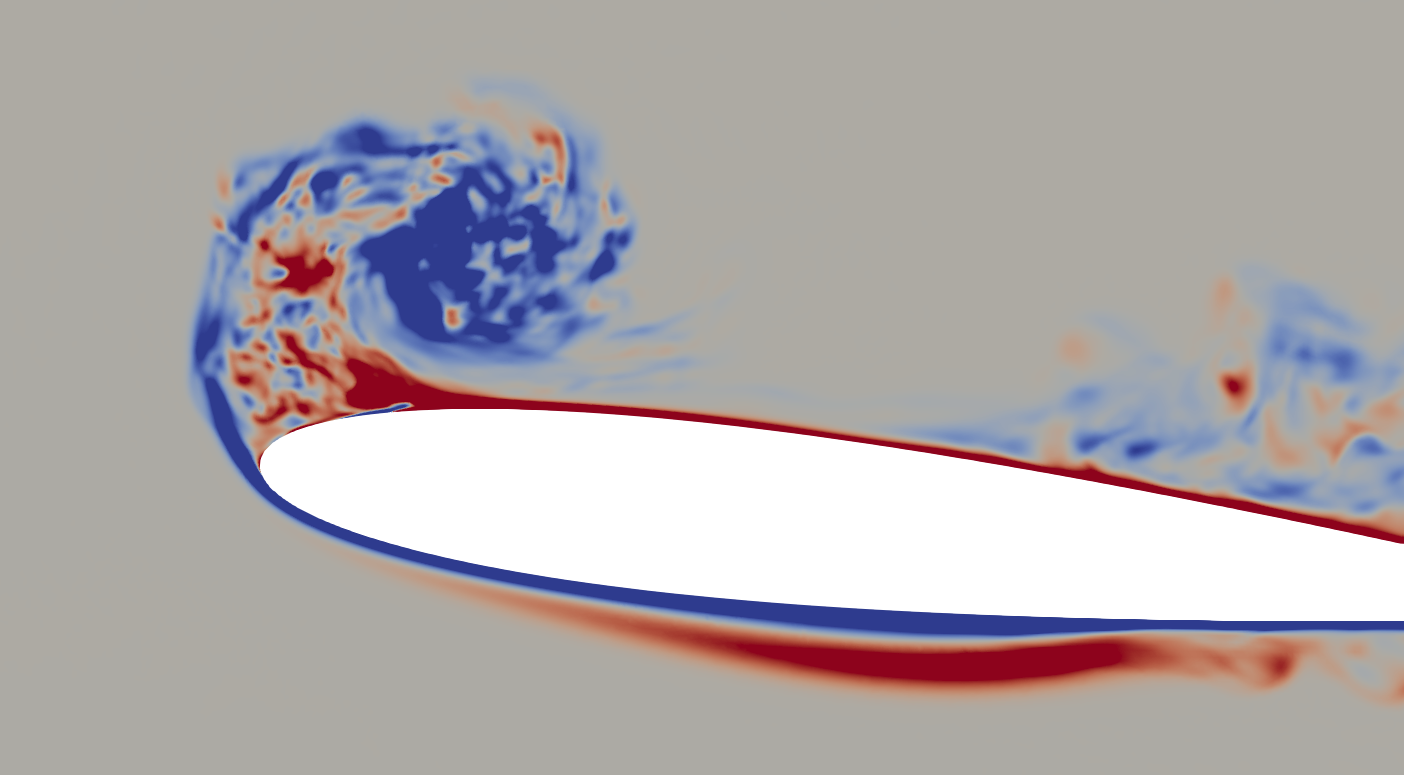
\includegraphics[width=1\textwidth]{figures/zonal_adapt_results/vorticity_plots/v2/Mza3_100/spavg/phase_240.png}
		\caption{Mza3\_100 mesh, $\psi$ = $240^\circ$}
		\label{fig:Mza3_100_sp_psi240}
	\end{subfigure}
	\caption{Spanwise vorticity comparison at $\psi$ = $240^\circ$ for different meshes}
	\label{fig:vorticity_sp_240}
\end{figure}

%%=====================================
%% Phase = 270
%%=====================================


\begin{figure}[H]
	\centering
	\begin{center}
		\begin{subfigure}[b]{0.475\textwidth}
		\centering
		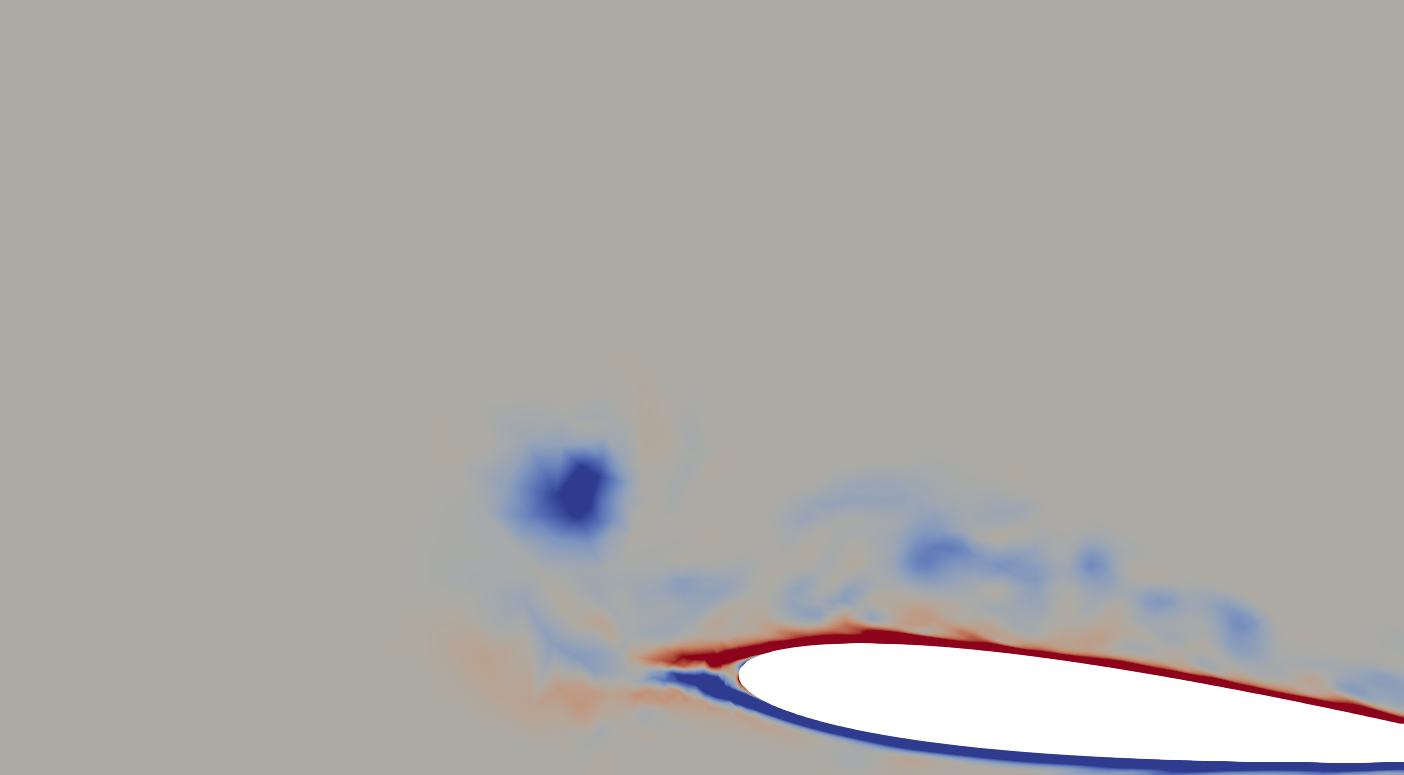
\includegraphics[width=1\textwidth]{figures/zonal_adapt_results/vorticity_plots/v3/M0/spavg/phase_270.png}
		\caption{M0 mesh, $\psi$ = $270^\circ$}
		\label{fig:M0_sp_psi270}
		\end{subfigure}
	\end{center}
	\begin{subfigure}[b]{0.475\textwidth}
	\centering
	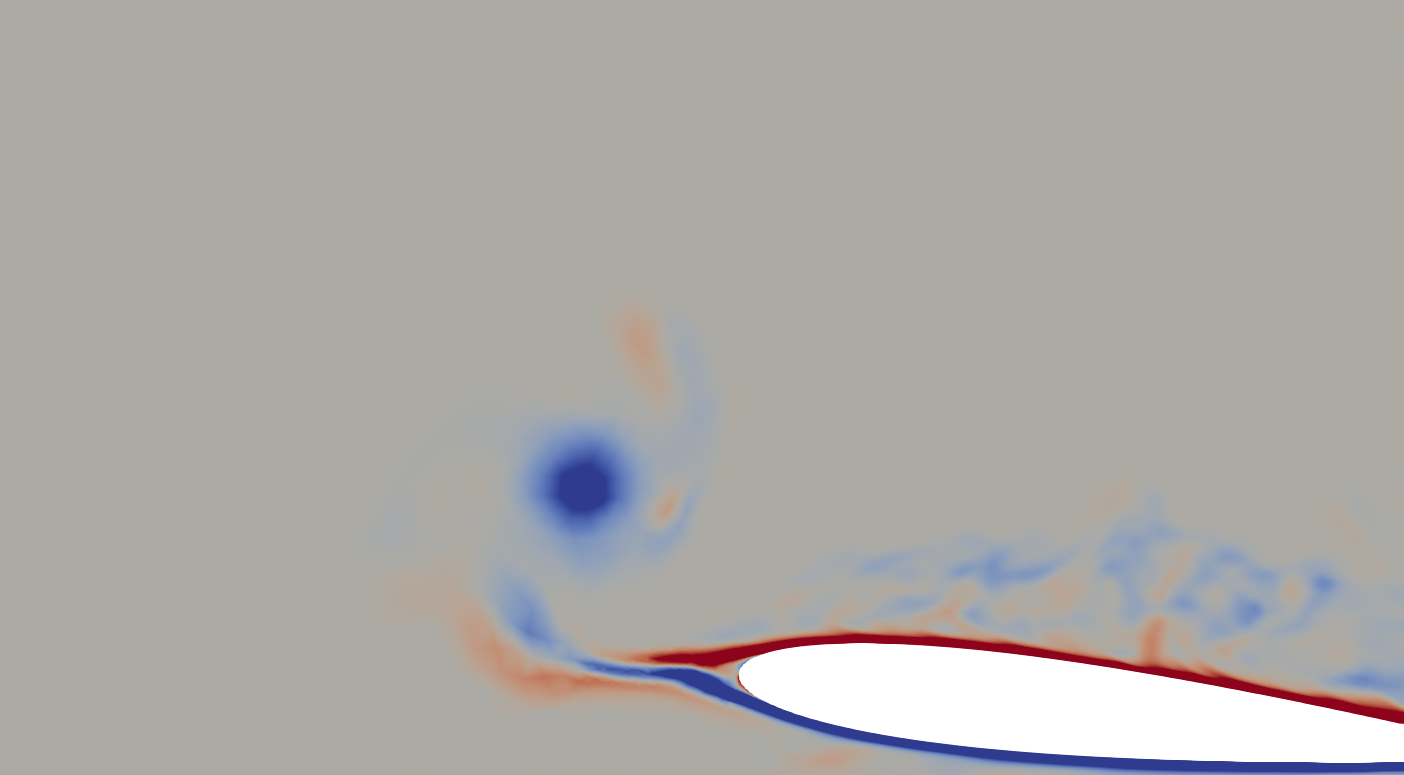
\includegraphics[width=1\textwidth]{figures/zonal_adapt_results/vorticity_plots/v3/Mza1_25/spavg/phase_270.png}
	\caption{Mza1\_25 mesh, $\psi$ = $270^\circ$}
	\label{fig:Mza1_25_sp_psi270}
	\end{subfigure}
	\begin{subfigure}[b]{0.475\textwidth}
		\centering
		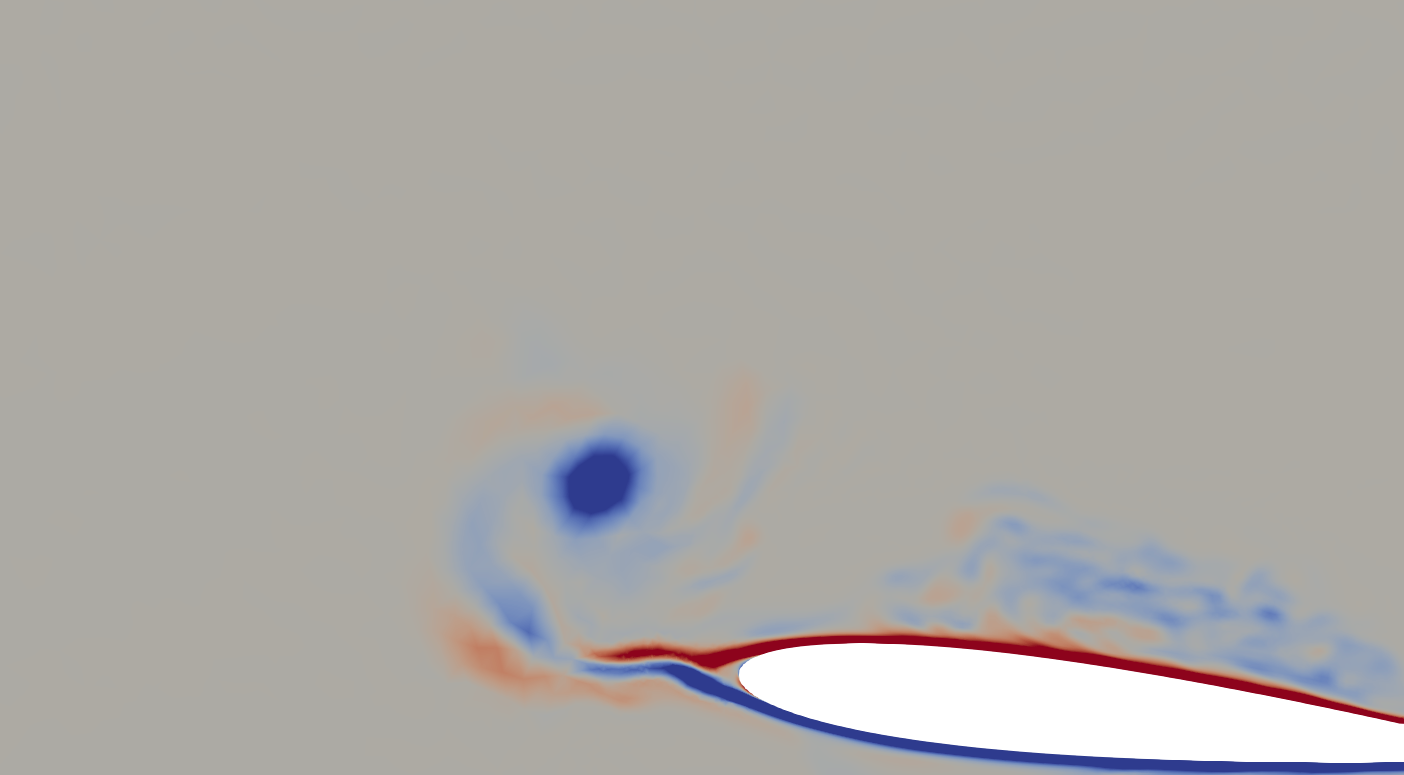
\includegraphics[width=1\textwidth]{figures/zonal_adapt_results/vorticity_plots/v3/Mza1_50/spavg/phase_270.png}
		\caption{Mza1\_50 mesh, $\psi$ = $270^\circ$}
		\label{fig:Mza1_50_sp_psi270}
	\end{subfigure}
%	\begin{subfigure}[b]{0.475\textwidth}
%		\centering
%		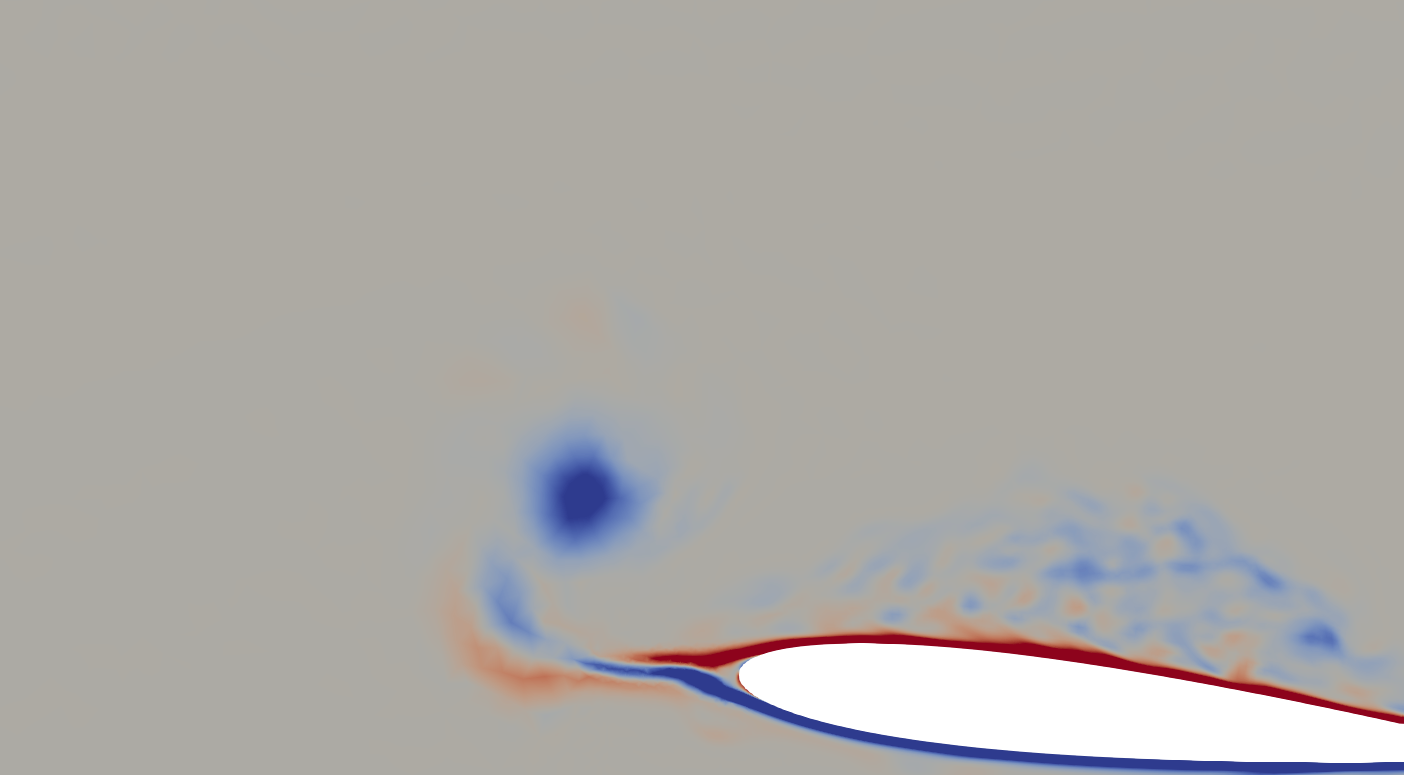
\includegraphics[width=1\textwidth]{figures/zonal_adapt_results/vorticity_plots/v3/Mza1_100/spavg/phase_270.png}
%		\caption{Mza1\_100 mesh, $\psi$ = $270^\circ$}
%		\label{fig:Mza1_100_sp_psi270}
%	\end{subfigure}
%	\begin{subfigure}[b]{0.475\textwidth}
%	\centering
%	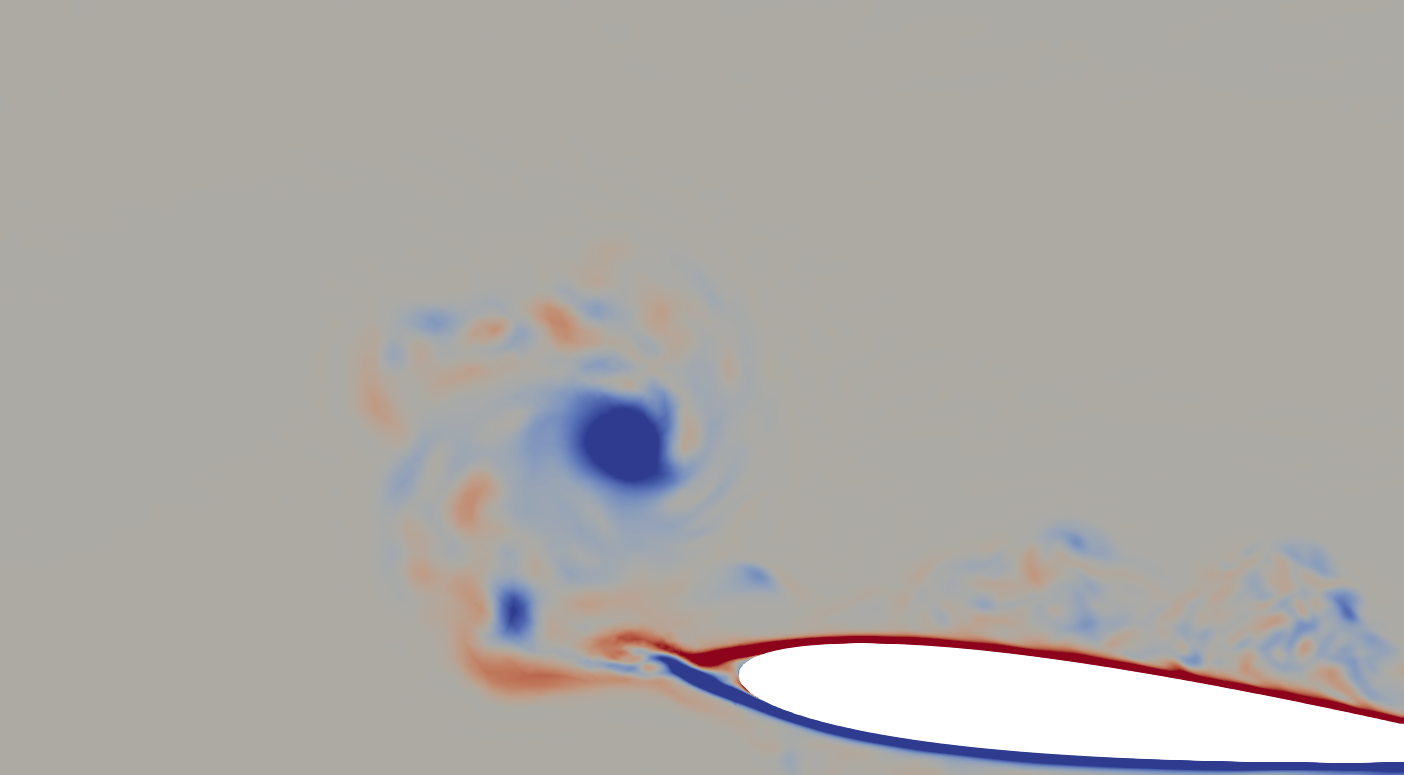
\includegraphics[width=1\textwidth]{figures/zonal_adapt_results/vorticity_plots/v3/Mza2_25/spavg/phase_270.png}
%	\caption{Mza2\_25 mesh, $\psi$ = $270^\circ$}
%	\label{fig:Mza2_25_sp_psi270}
%    \end{subfigure}	
	\begin{subfigure}[b]{0.475\textwidth}
		\centering
		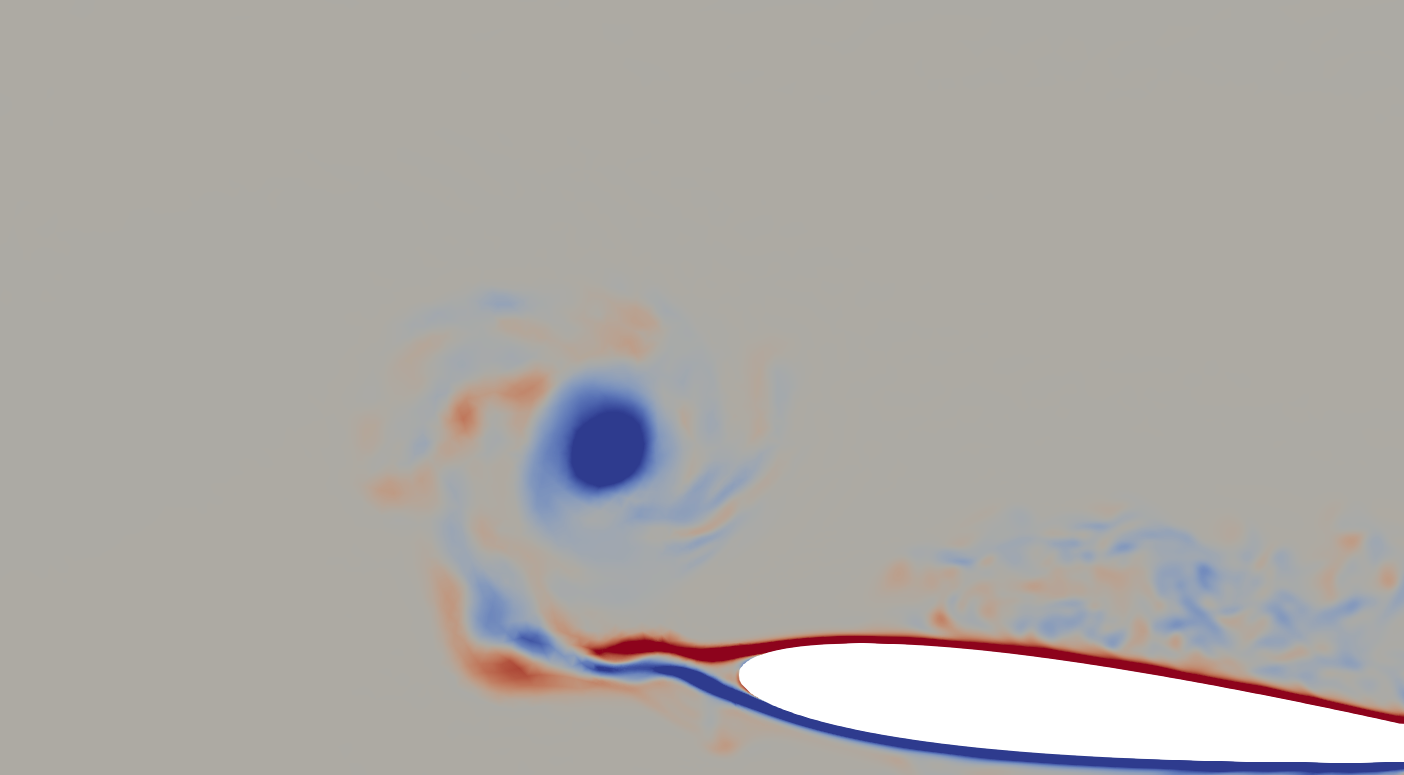
\includegraphics[width=1\textwidth]{figures/zonal_adapt_results/vorticity_plots/v3/Mza2_50/spavg/phase_270.png}
		\caption{Mza2\_50 mesh, $\psi$ = $270^\circ$}
		\label{fig:Mza2_50_sp_psi270}
	\end{subfigure}	
	\begin{subfigure}[b]{0.475\textwidth}
		\centering
		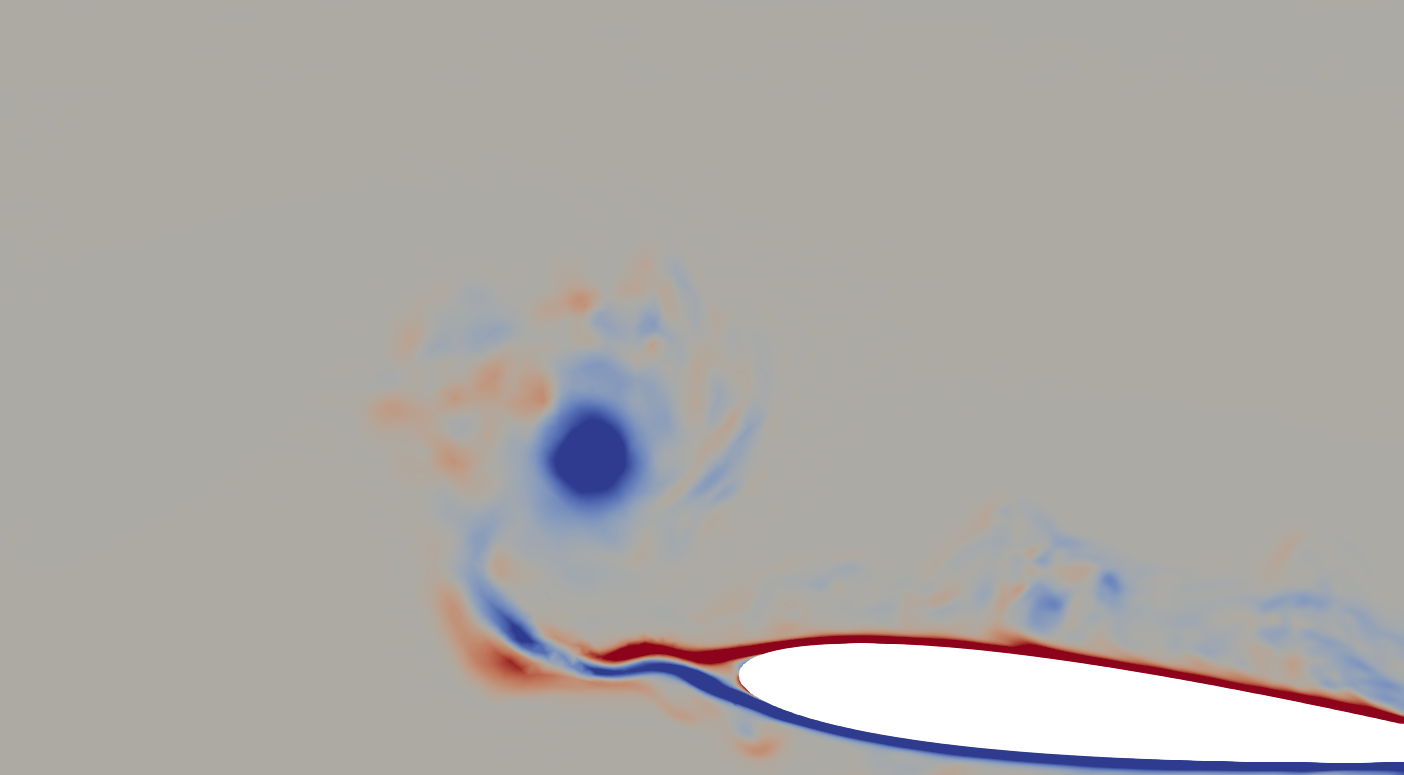
\includegraphics[width=1\textwidth]{figures/zonal_adapt_results/vorticity_plots/v3/Mza2_100/spavg/phase_270.png}
		\caption{Mza2\_100 mesh, $\psi$ = $270^\circ$}
		\label{fig:Mza2_100_sp_psi270}
	\end{subfigure}
	\begin{subfigure}[b]{0.475\textwidth}
	\centering
	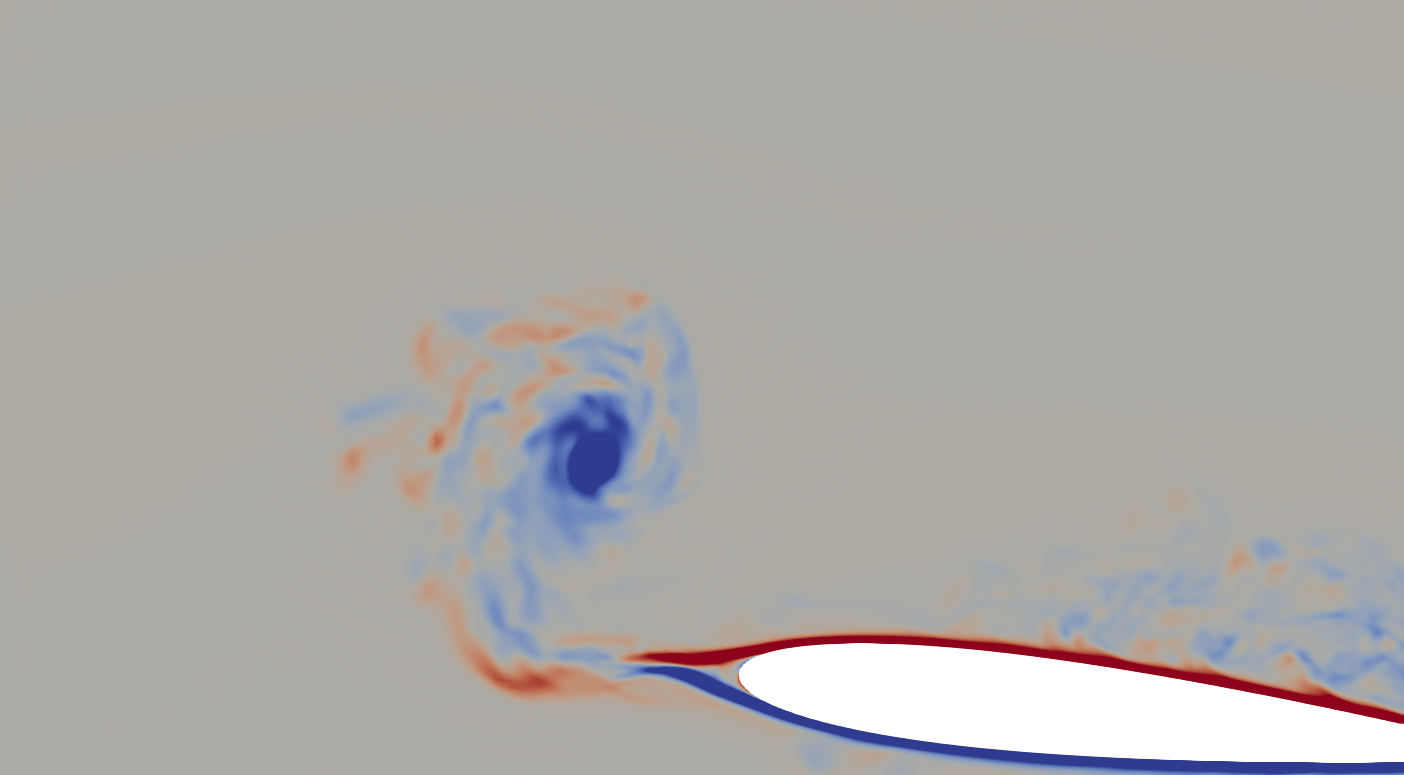
\includegraphics[width=1\textwidth]{figures/zonal_adapt_results/vorticity_plots/v3/Mza3_50/spavg/phase_270.png}
	\caption{Mza3\_50 mesh, $\psi$ = $270^\circ$}
	\label{fig:Mza3_50_sp_psi270}
\end{subfigure}
	\begin{subfigure}[b]{0.475\textwidth}
		\centering
		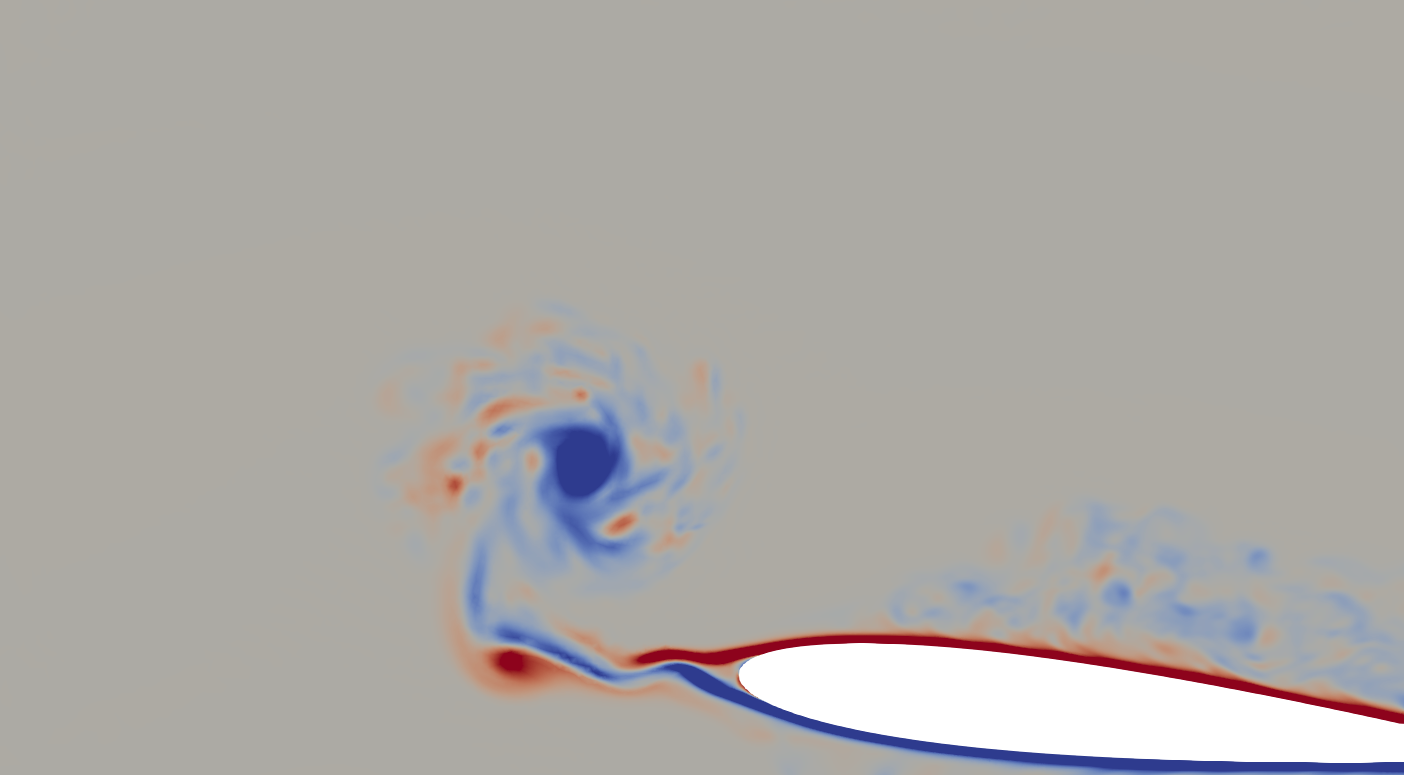
\includegraphics[width=1\textwidth]{figures/zonal_adapt_results/vorticity_plots/v3/Mza3_100/spavg/phase_270.png}
		\caption{Mza3\_100 mesh, $\psi$ = $270^\circ$}
		\label{fig:Mza3_100_sp_psi270}
	\end{subfigure}
	\caption{Spanwise vorticity comparison at $\psi$ = $270^\circ$ for different meshes}
	\label{fig:vorticity_sp_270}
\end{figure}

\begin{comment}


\begin{figure}[H]
	\centering
	\begin{subfigure}[b]{0.475\textwidth}
		\centering
		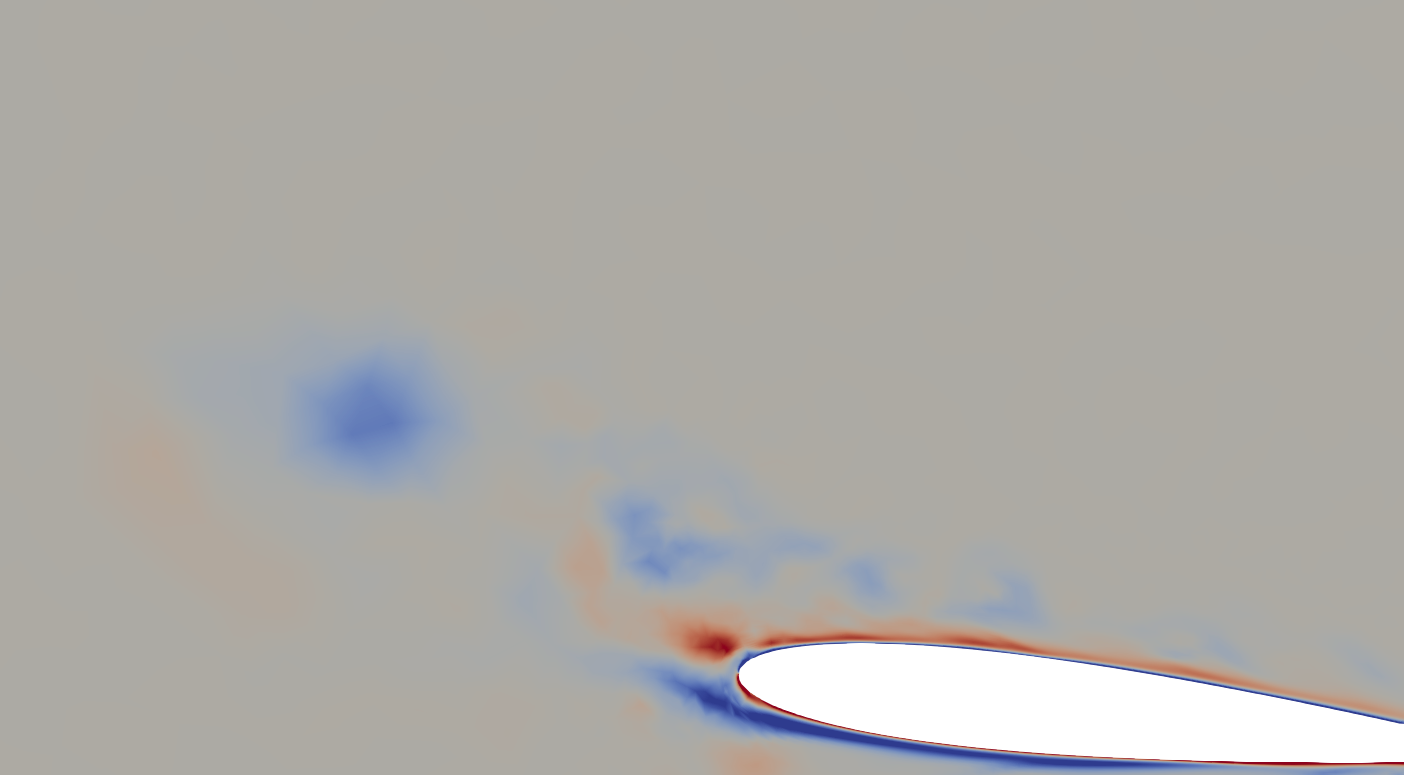
\includegraphics[width=1\textwidth]{figures/zonal_adapt_results/vorticity_plots/v3/M0/spavg/phase_300.png}
		\caption{M0 mesh, $\psi$ = $300^\circ$}
		\label{fig:M0_sp_psi300}
	\end{subfigure}
	\begin{subfigure}[b]{0.475\textwidth}
	\centering
	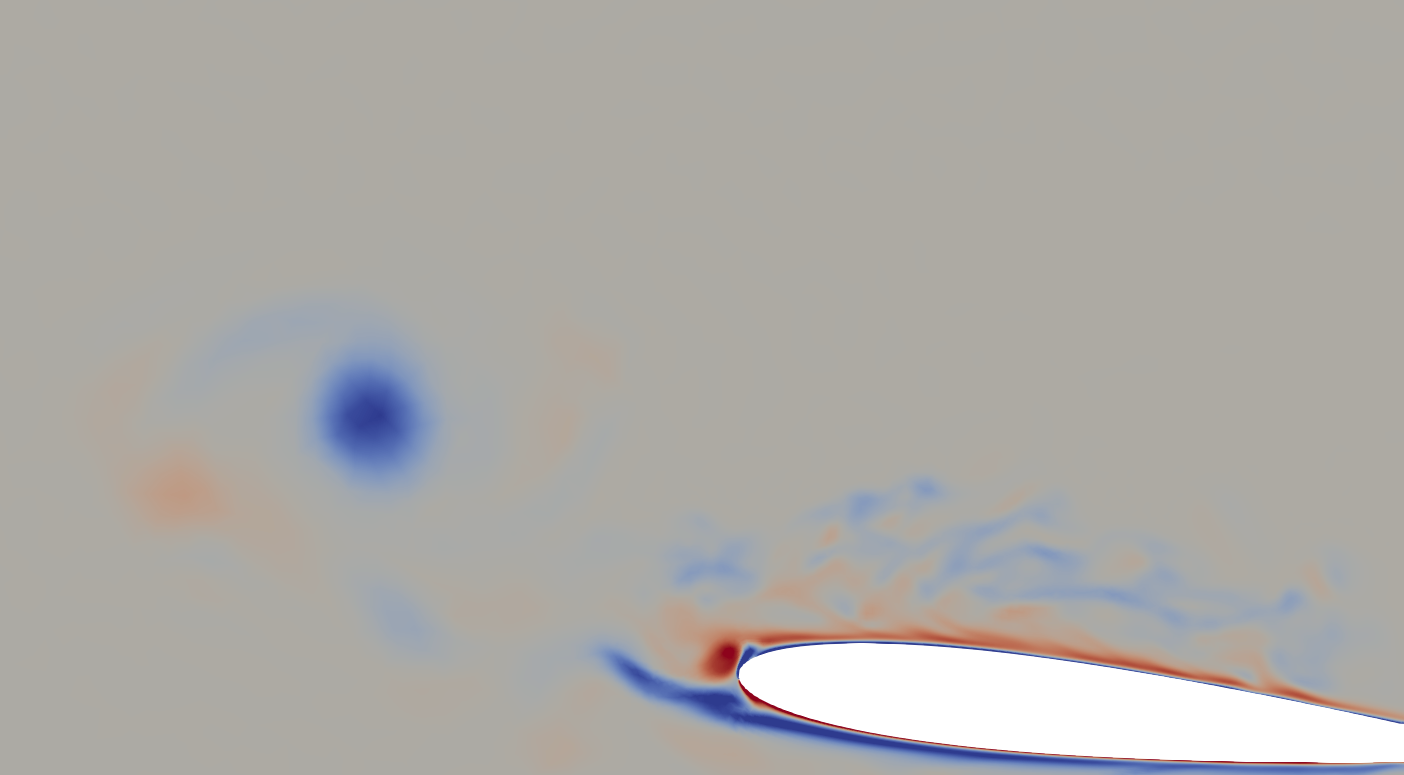
\includegraphics[width=1\textwidth]{figures/zonal_adapt_results/vorticity_plots/v3/Mza1_25/spavg/phase_300.png}
	\caption{Mza1\_25 mesh, $\psi$ = $300^\circ$}
	\label{fig:Mza1_25_sp_psi300}
	\end{subfigure}
	\begin{subfigure}[b]{0.475\textwidth}
		\centering
		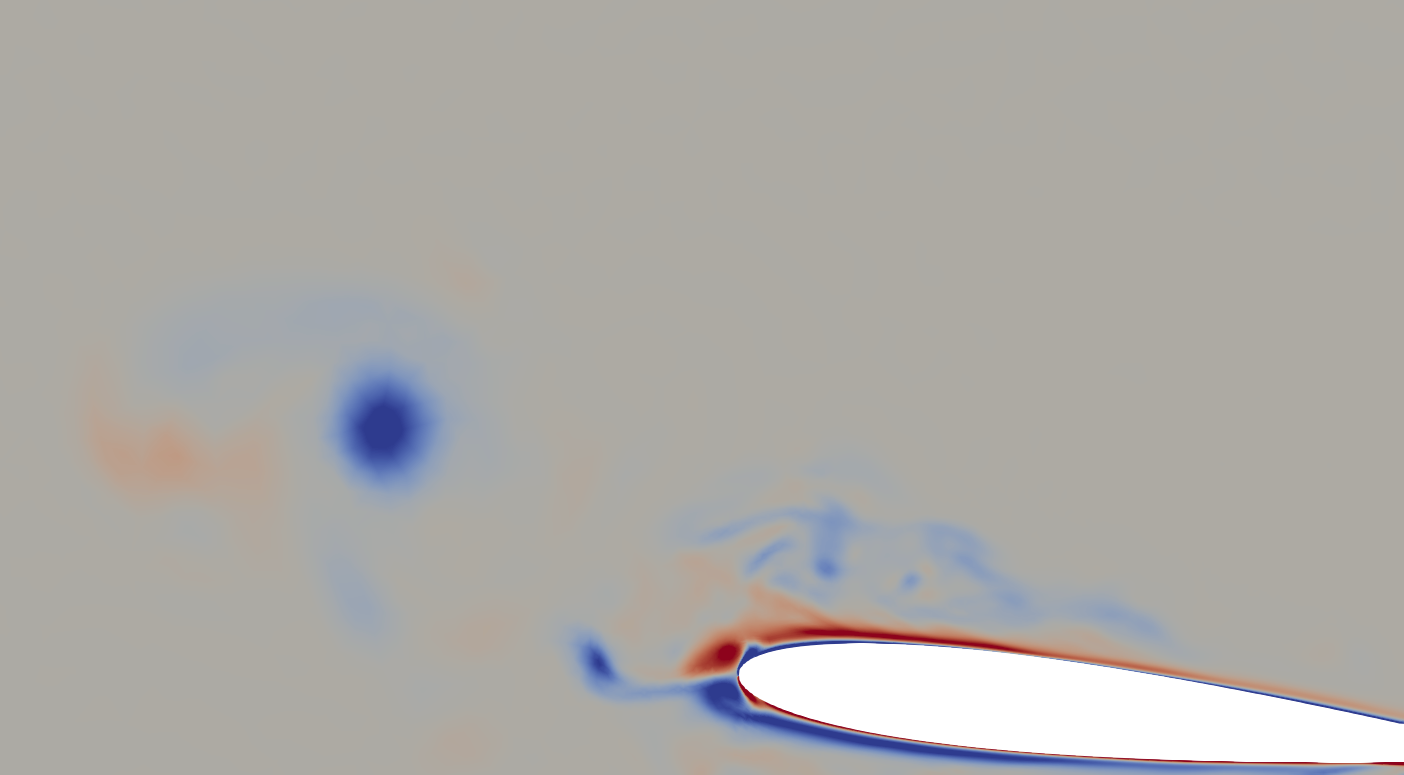
\includegraphics[width=1\textwidth]{figures/zonal_adapt_results/vorticity_plots/v3/Mza1_50/spavg/phase_300.png}
		\caption{Mza1\_50 mesh, $\psi$ = $300^\circ$}
		\label{fig:Mza1_50_sp_psi300}
	\end{subfigure}
%	\begin{subfigure}[b]{0.475\textwidth}
%		\centering
%		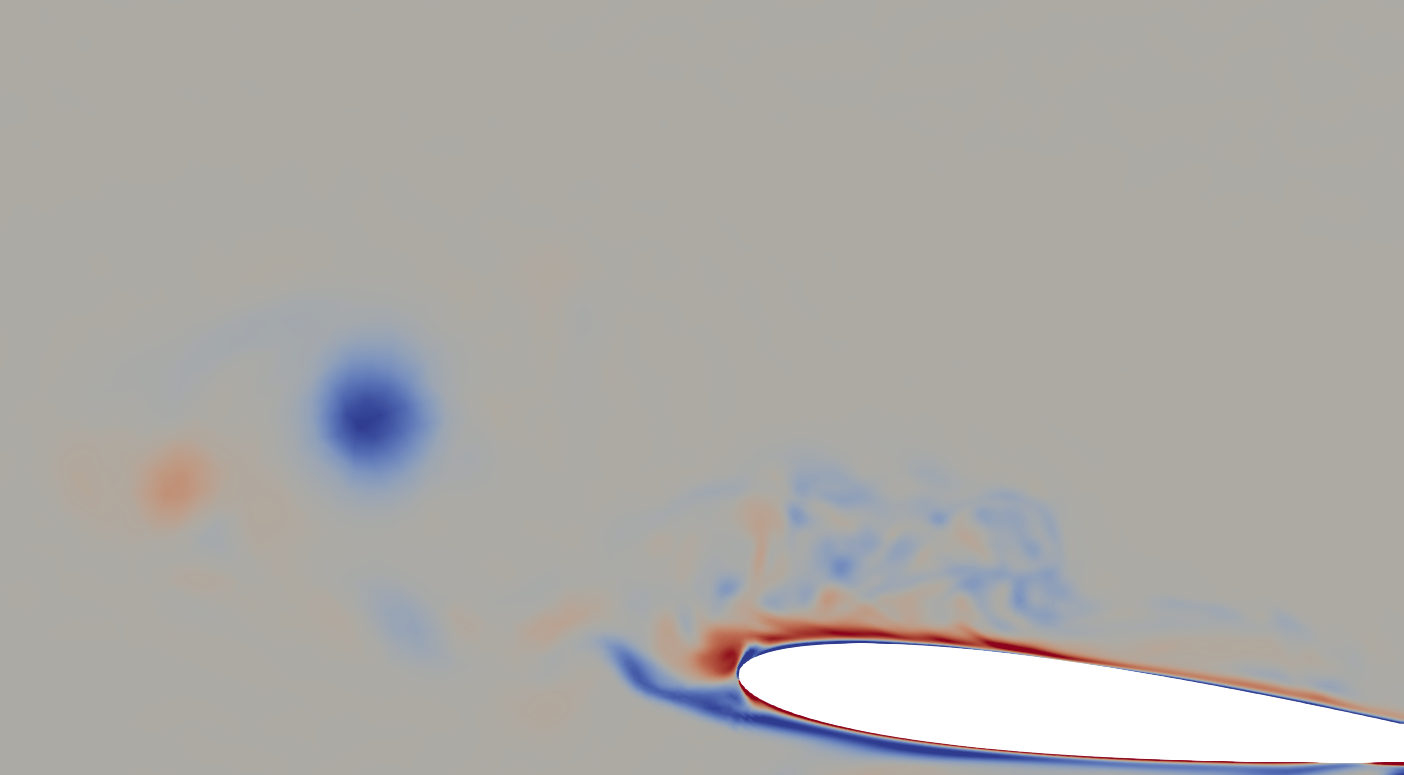
\includegraphics[width=1\textwidth]{figures/zonal_adapt_results/vorticity_plots/v3/Mza1_100/spavg/phase_300.png}
%		\caption{Mza1\_100 mesh, $\psi$ = $300^\circ$}
%		\label{fig:Mza1_100_sp_psi300}
%	\end{subfigure}
	\begin{subfigure}[b]{0.475\textwidth}
	\centering
	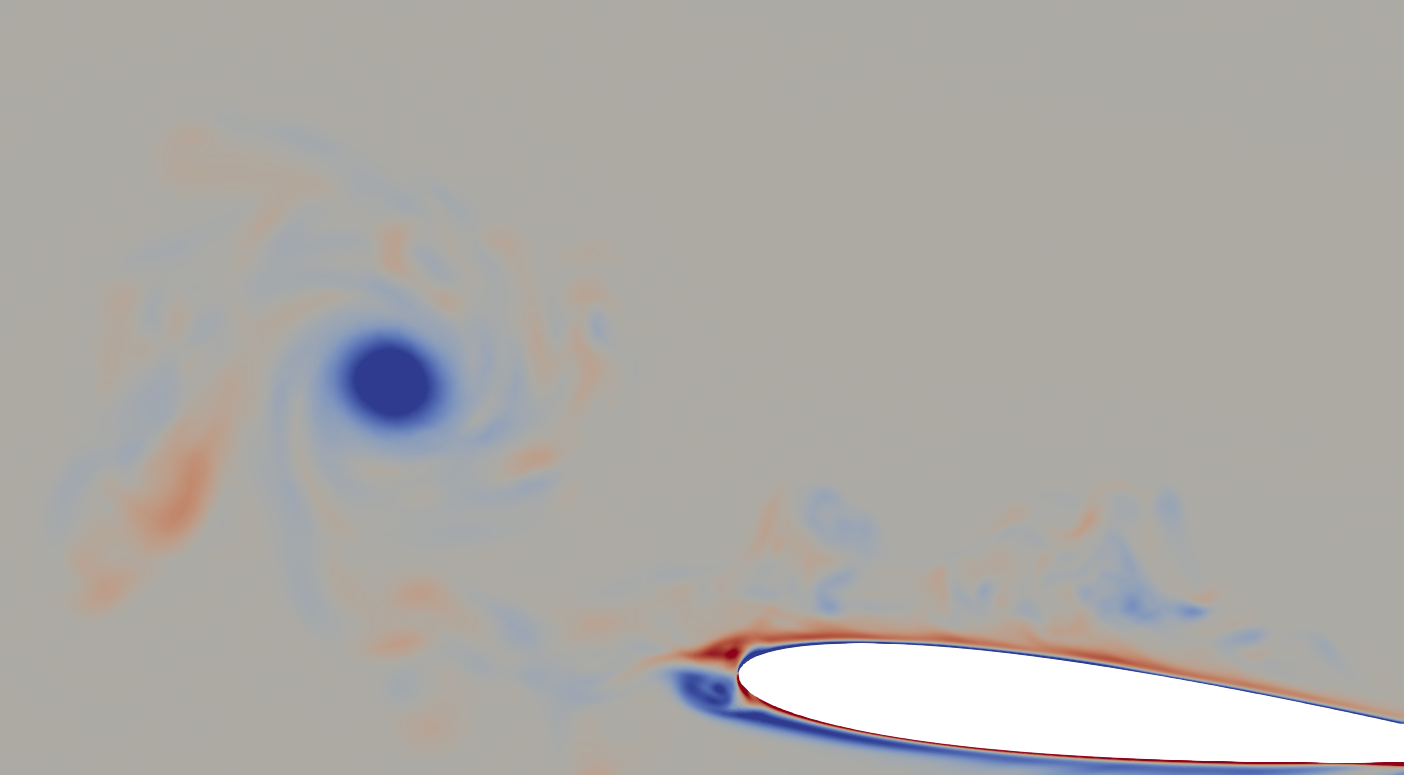
\includegraphics[width=1\textwidth]{figures/zonal_adapt_results/vorticity_plots/v3/Mza2_25/spavg/phase_300.png}
	\caption{Mza2\_25 mesh, $\psi$ = $300^\circ$}
	\label{fig:Mza2_25_sp_psi300}
\end{subfigure}	
	\begin{subfigure}[b]{0.475\textwidth}
		\centering
		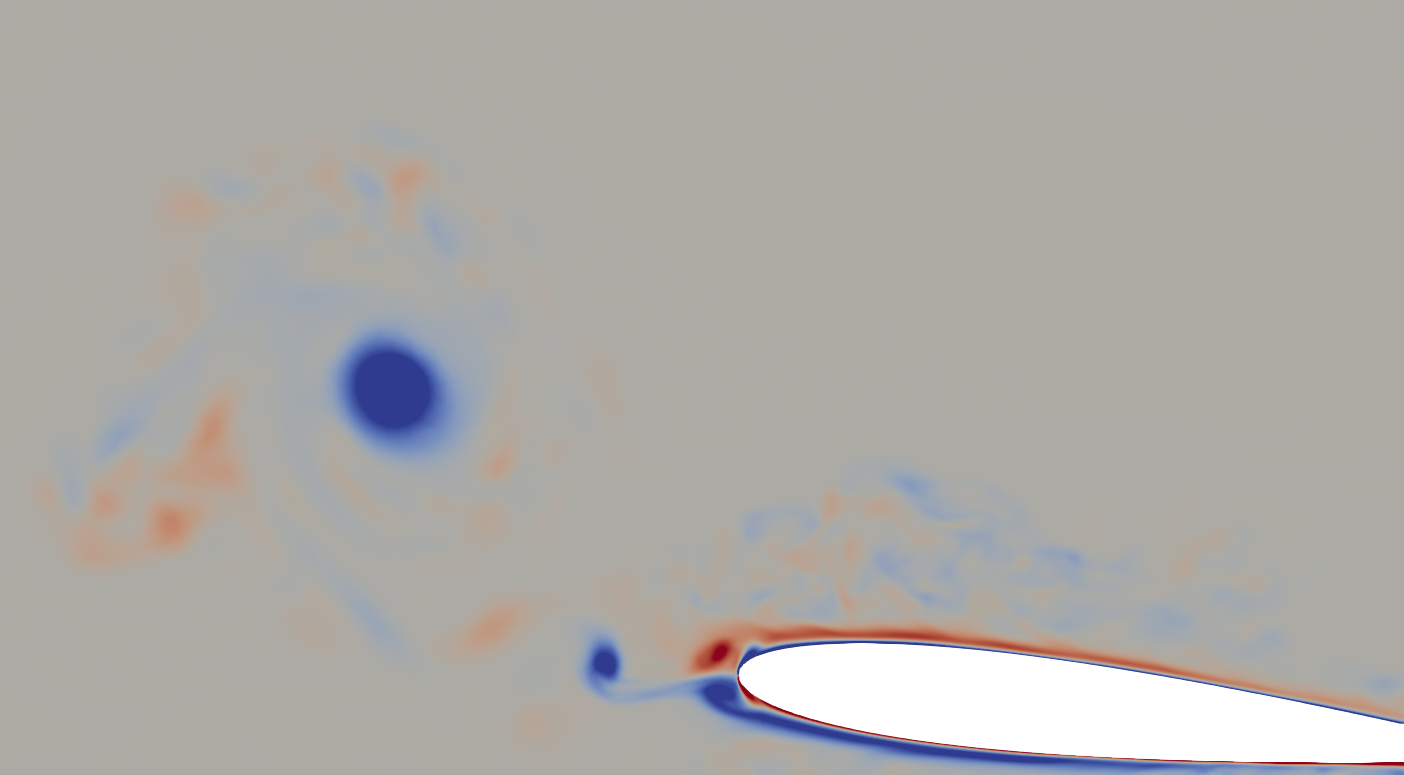
\includegraphics[width=1\textwidth]{figures/zonal_adapt_results/vorticity_plots/v3/Mza2_50/spavg/phase_300.png}
		\caption{Mza2\_50 mesh, $\psi$ = $300^\circ$}
		\label{fig:Mza2_50_sp_psi300}
	\end{subfigure}	
	\begin{subfigure}[b]{0.475\textwidth}
		\centering
		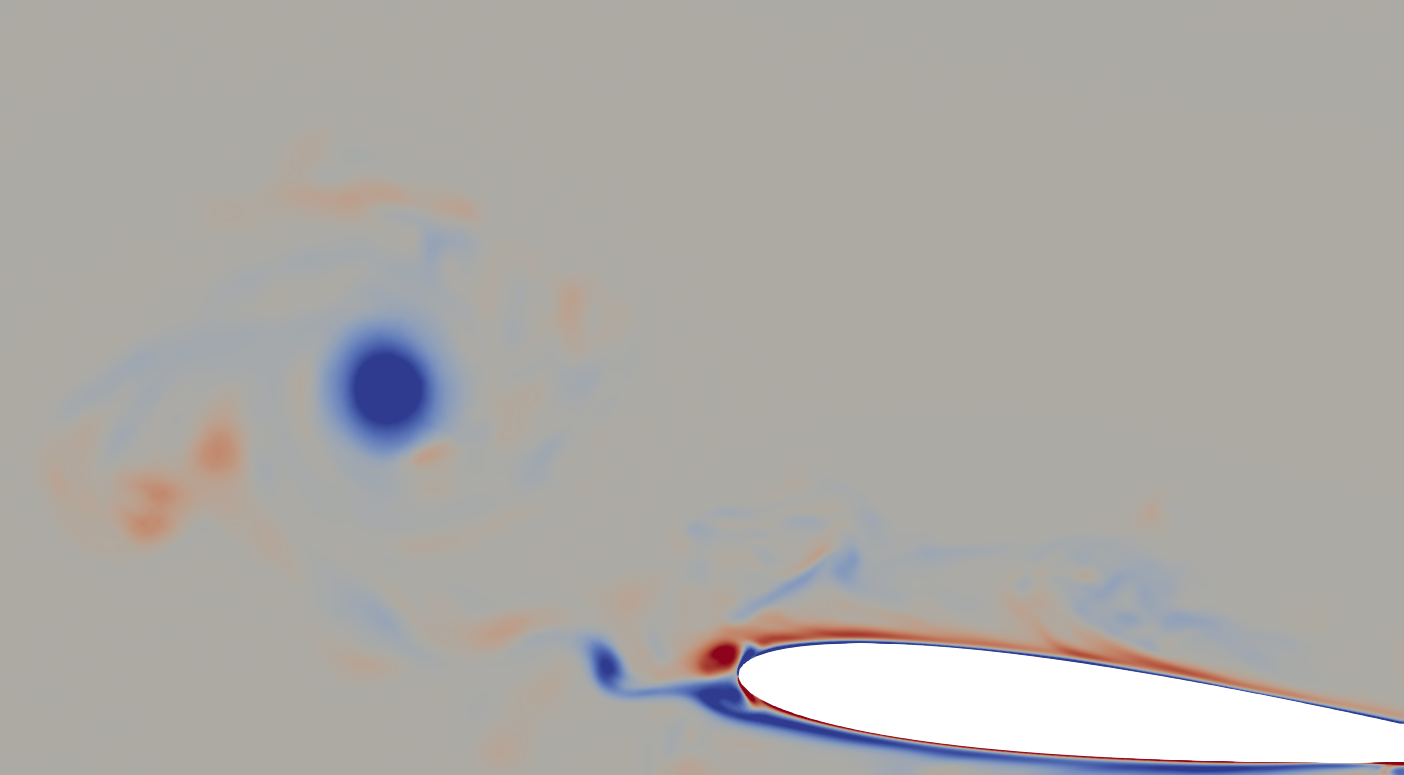
\includegraphics[width=1\textwidth]{figures/zonal_adapt_results/vorticity_plots/v3/Mza2_100/spavg/phase_300.png}
		\caption{Mza2\_100 mesh, $\psi$ = $300^\circ$}
		\label{fig:Mza2_100_sp_psi300}
	\end{subfigure}
	\begin{subfigure}[b]{0.475\textwidth}
	\centering
	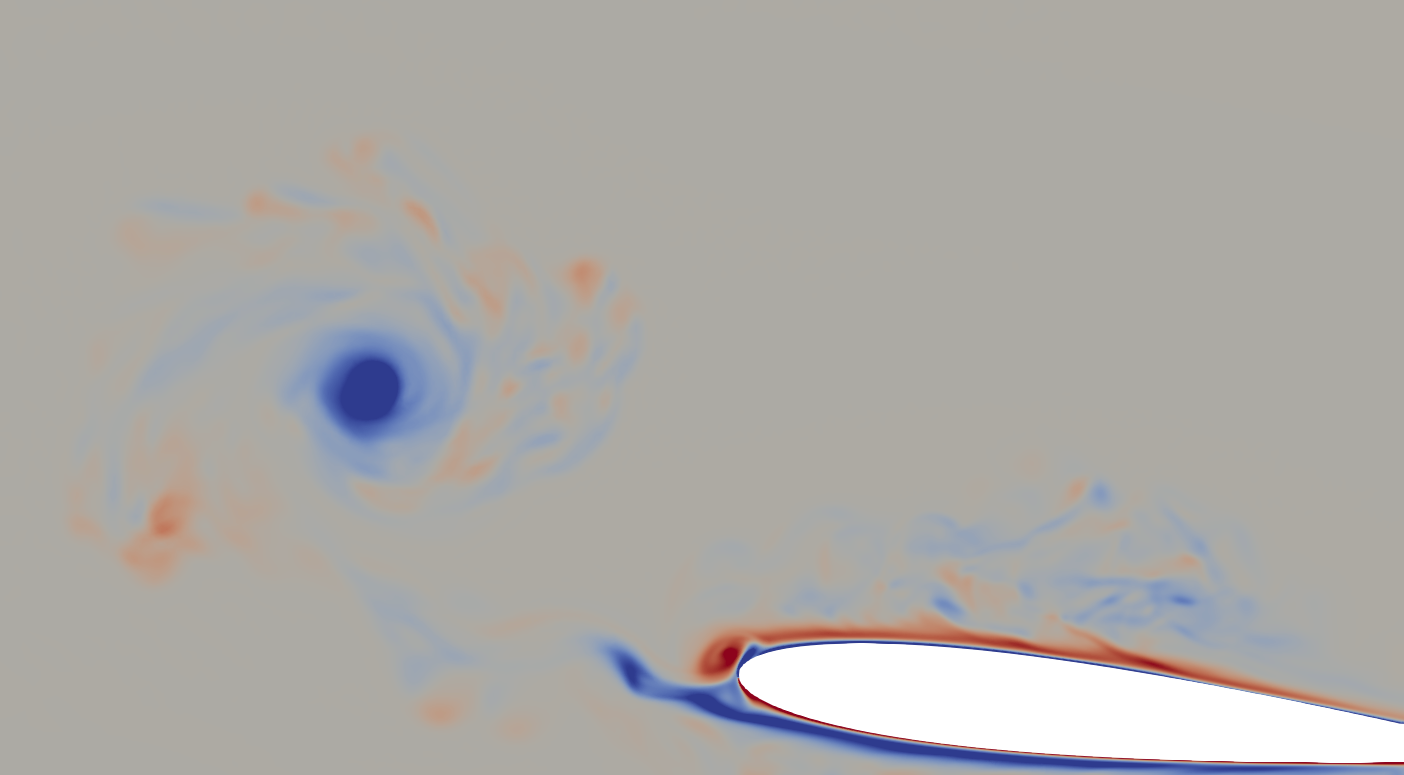
\includegraphics[width=1\textwidth]{figures/zonal_adapt_results/vorticity_plots/v3/Mza3_50/spavg/phase_300.png}
	\caption{Mza3\_50 mesh, $\psi$ = $300^\circ$}
	\label{fig:Mza3_50_sp_psi300}
\end{subfigure}
	\begin{subfigure}[b]{0.475\textwidth}
		\centering
		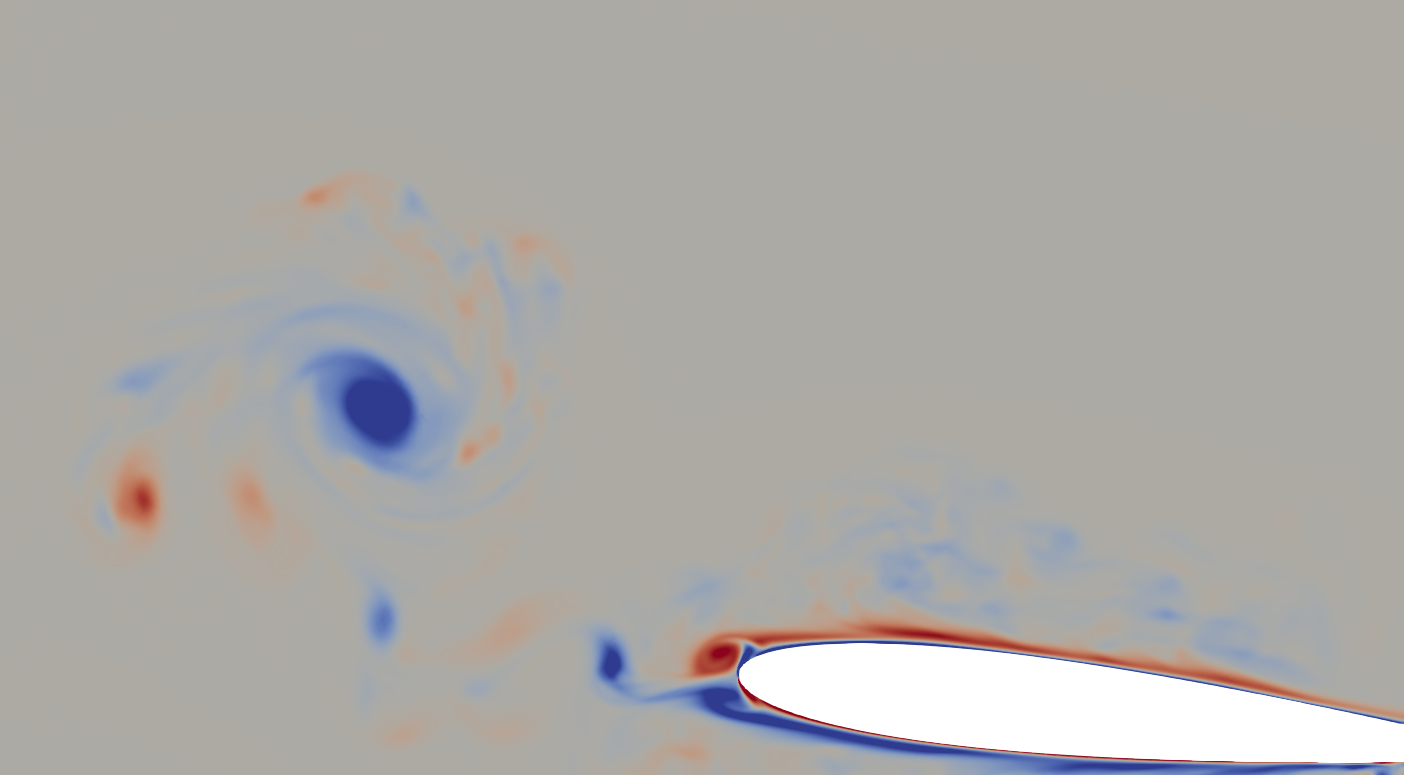
\includegraphics[width=1\textwidth]{figures/zonal_adapt_results/vorticity_plots/v3/Mza3_100/spavg/phase_300.png}
		\caption{Mza3\_100 mesh, $\psi$ = $300^\circ$}
		\label{fig:Mza3_100_sp_psi300}
	\end{subfigure}
	\caption{Spanwise vorticity comparison at $\psi$ = $300^\circ$ for different meshes}
	\label{fig:vorticity_sp_300}
\end{figure}

\end{comment}
